\documentclass[a4paper]{article}

\usepackage[english]{babel}
\usepackage[utf8]{inputenc}
\usepackage{amsmath}
\usepackage{graphicx}
\usepackage[colorinlistoftodos]{todonotes}
\usepackage{caption}
\usepackage{subcaption}
\usepackage{here}

\title{Computational Photography \\ Project 1, Fall 2014}

\author{Mich\`ele Wyss, 10-104-123}

\date{October 2, 2014}

\graphicspath{{imgs/}}
\begin{document}
\maketitle
\section{The Spanish Castle illusion}
The Spanish Castle illusion is an astonishing effect to demonstrate how the human eye can be influenced by temporal effects.  In the 19$^{\text{th}}$ century, the so-called \emph{Opponent process theory} was proposed. According to this theory, the color perception of a human eye is controlled by ``encoding'' colors as red vs.\ green,  blue vs.\ yellow and black vs.\ white. Further, the theory states that there are two types of chemical reactions, namely \emph{anabolic} and \emph{catabolic} processes. For simplicity, one could understand them as ``positive'' or ``negative'' reactions. The processes are in a sense the opposite of each other. The positive reaction yields one member of an opponent pair, whereas the negative reaction yields the other one. An anabolic process requires energy and a catabolic one releases energy. If a stimulus of a certain color is given, then the corresponding process will be reversed after the stimulus is removed again, and this will give the impression of perceiving the opposite color.
\section*{Example images}
\begin{figure}[H]
	%\centering
	\begin{subfigure}[h]{0.24\textwidth}
		\centering
		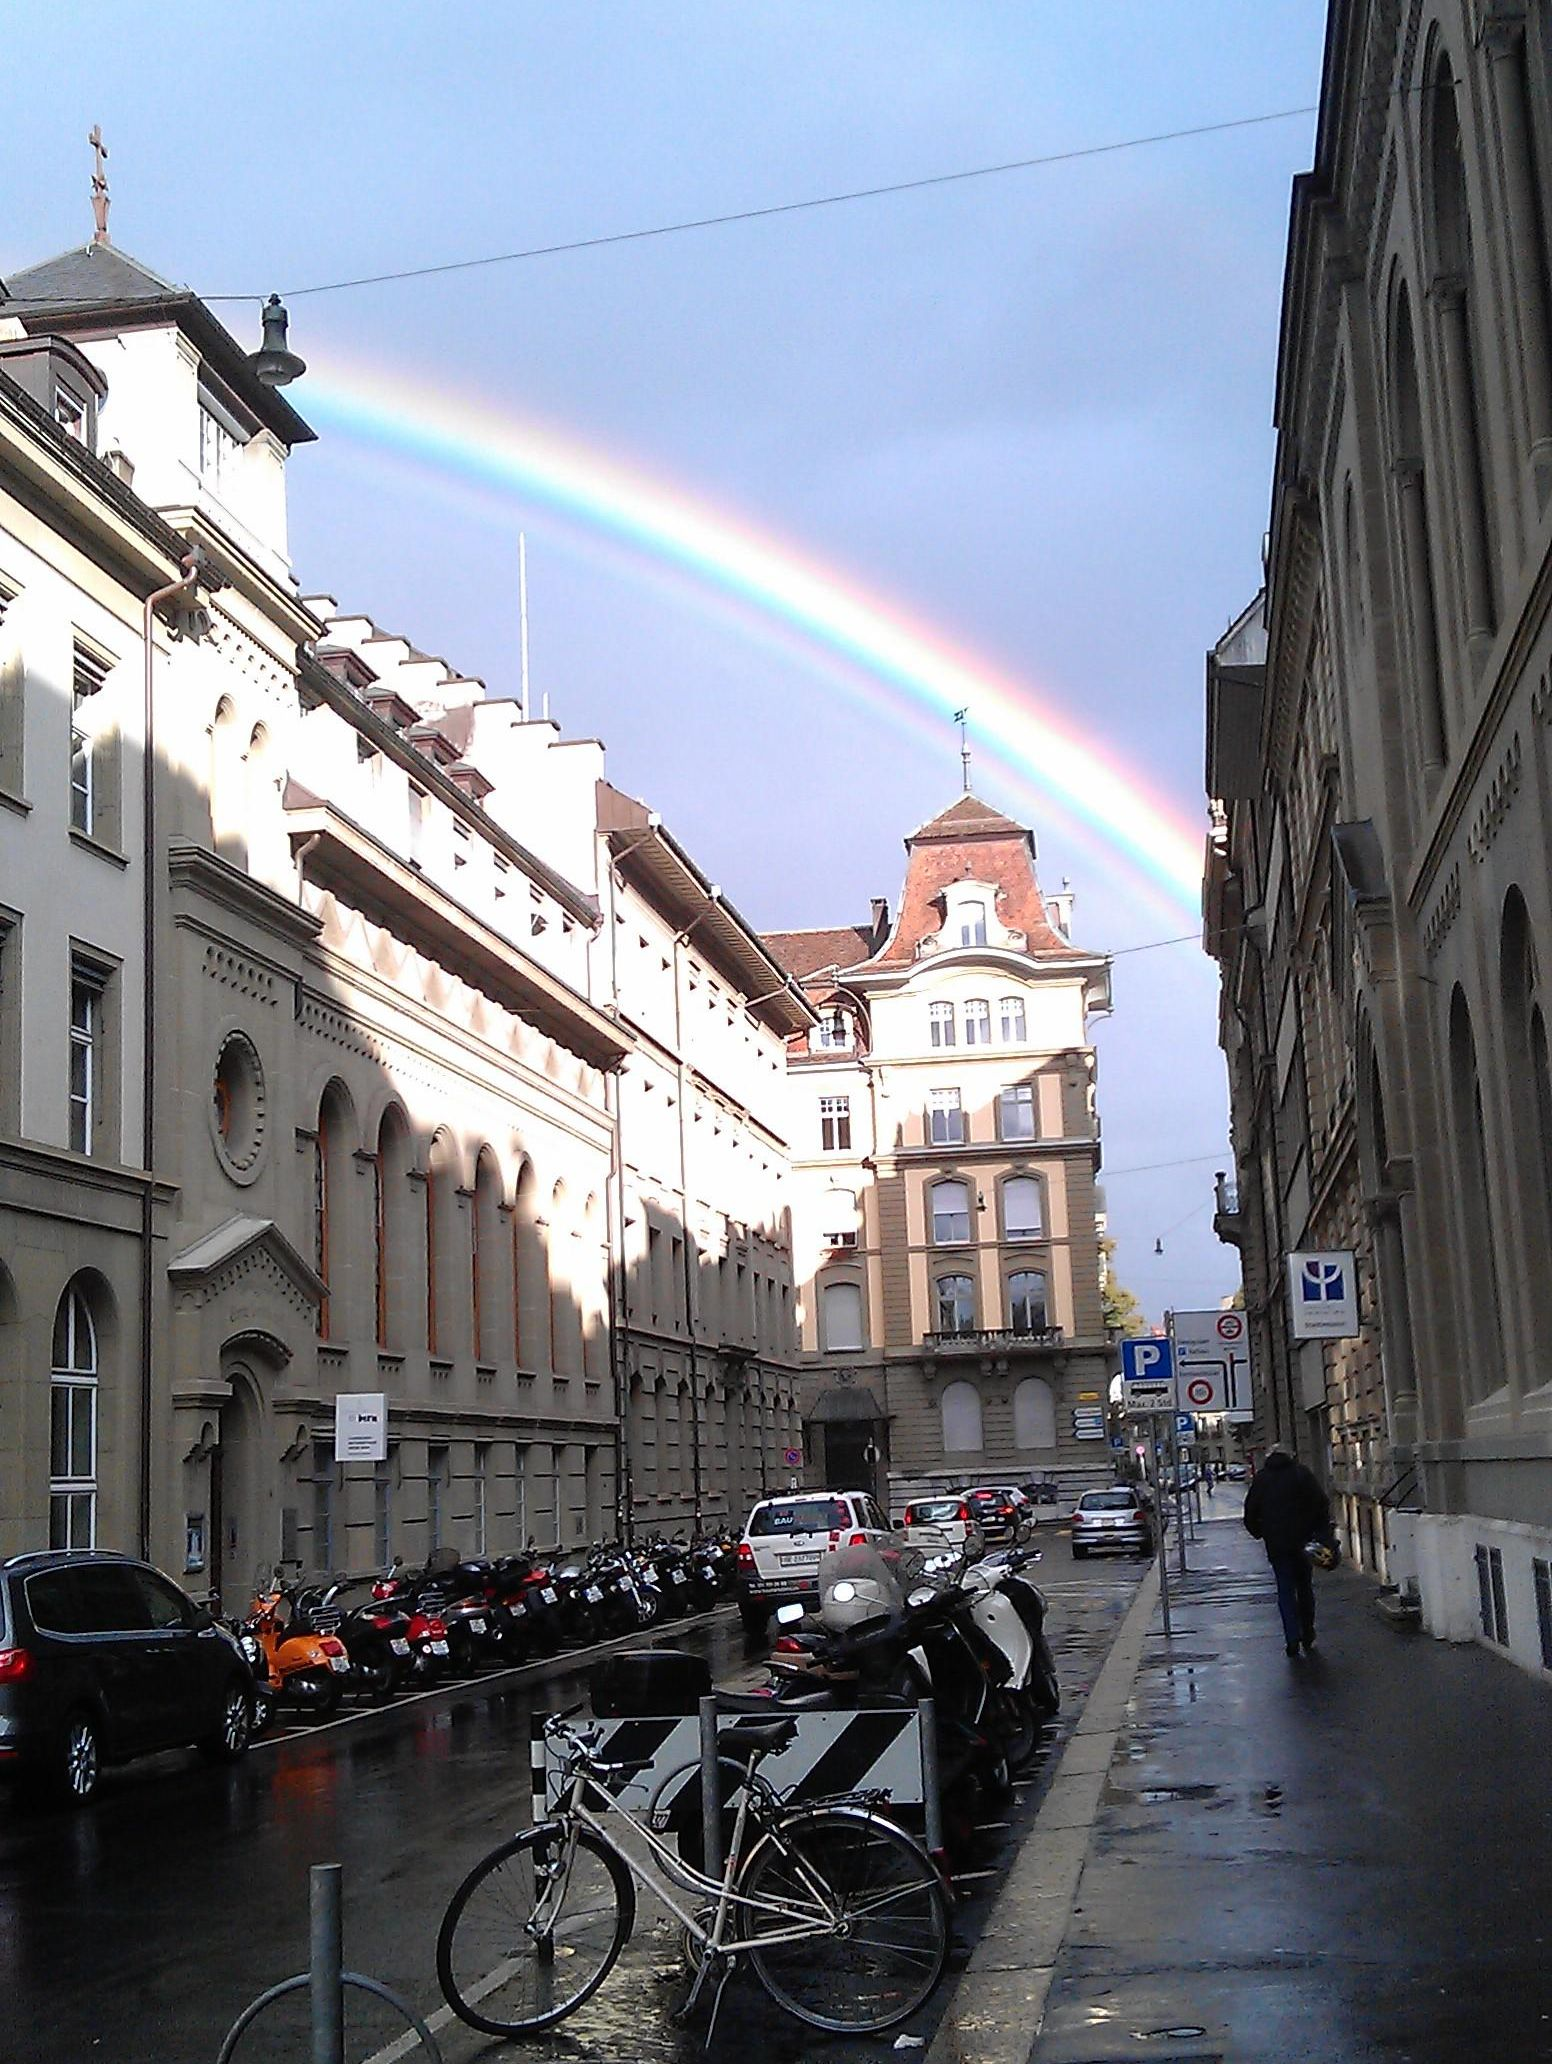
\includegraphics[width=\textwidth]{rainbow}
		\caption*{Input image}
	\end{subfigure}
	
	\vspace{3mm}
	\begin{subfigure}[h]{0.48\textwidth}
		\centering
		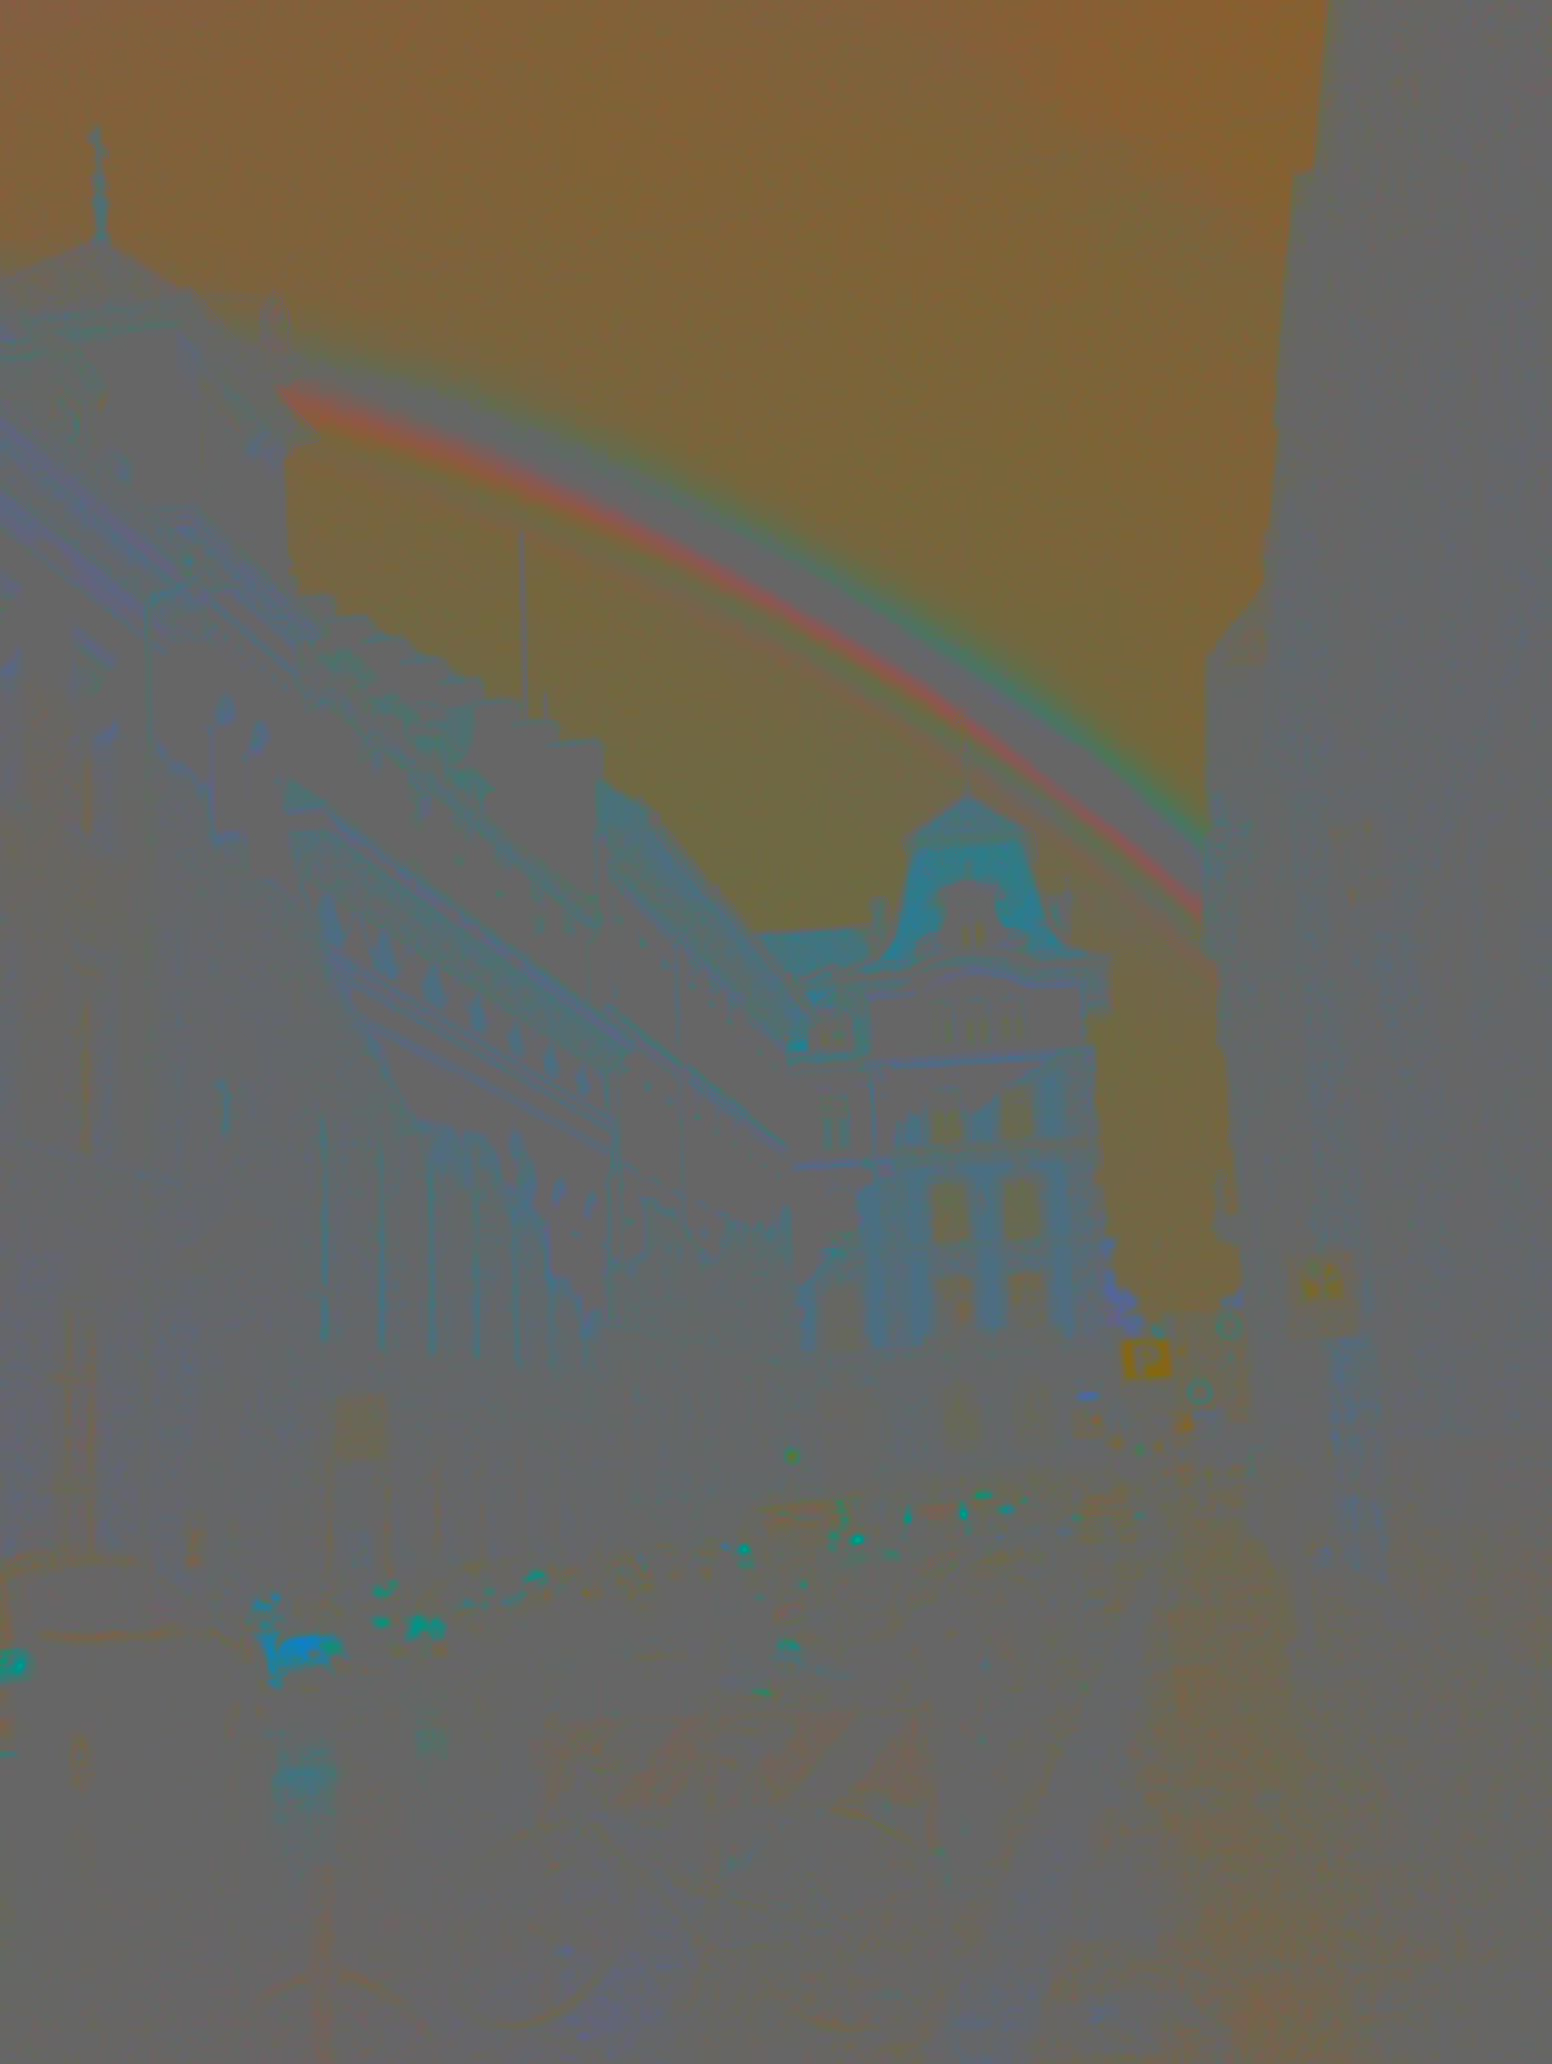
\includegraphics[width=\textwidth]{rainbow_inv}
		\caption*{Inverted image}
	\end{subfigure}
	~
	\begin{subfigure}[h]{0.48\textwidth}
		\centering
		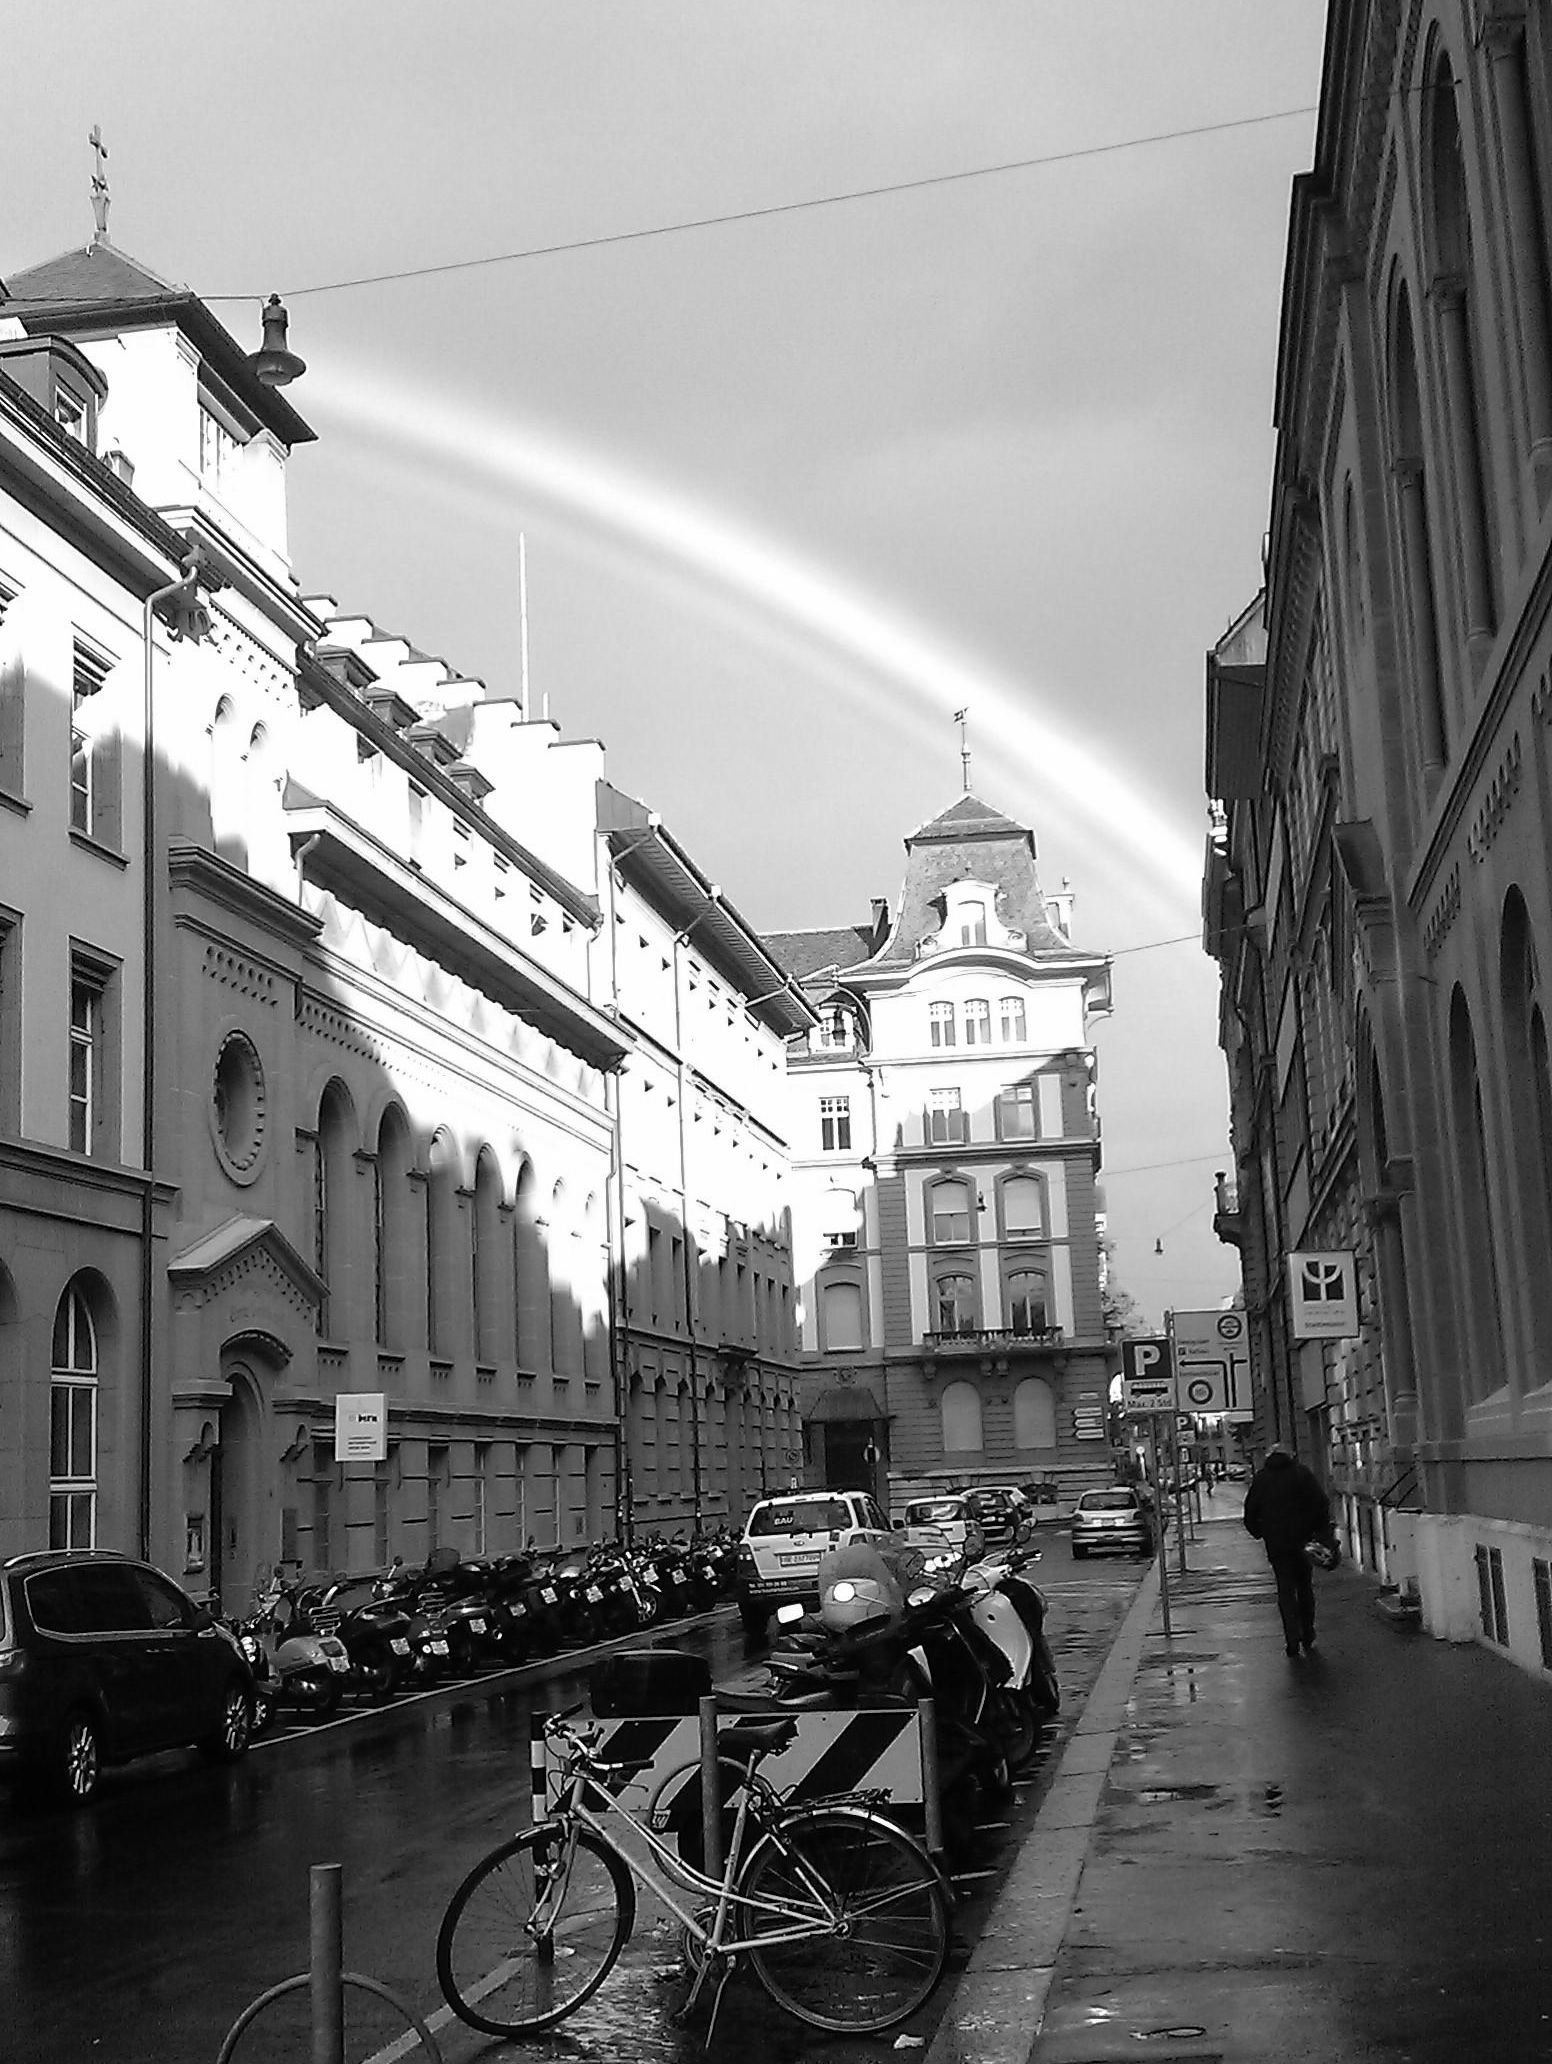
\includegraphics[width=\textwidth]{rainbow_gray}
		\caption*{Gray-scale image}
	\end{subfigure}	
\caption{The spanish castle illusion with the example of a photograph with a rainbow captured in Bern in September 2013. Starring at the inverted image long enough and then at the gray-scale image will produce the astonishing effect of perceiving the original colors in the gray-scale image.}
\label{fig:rainbow}
\end{figure}

\begin{figure}[H]
	%\centering
	\begin{subfigure}[h]{0.24\textwidth}
		\centering
		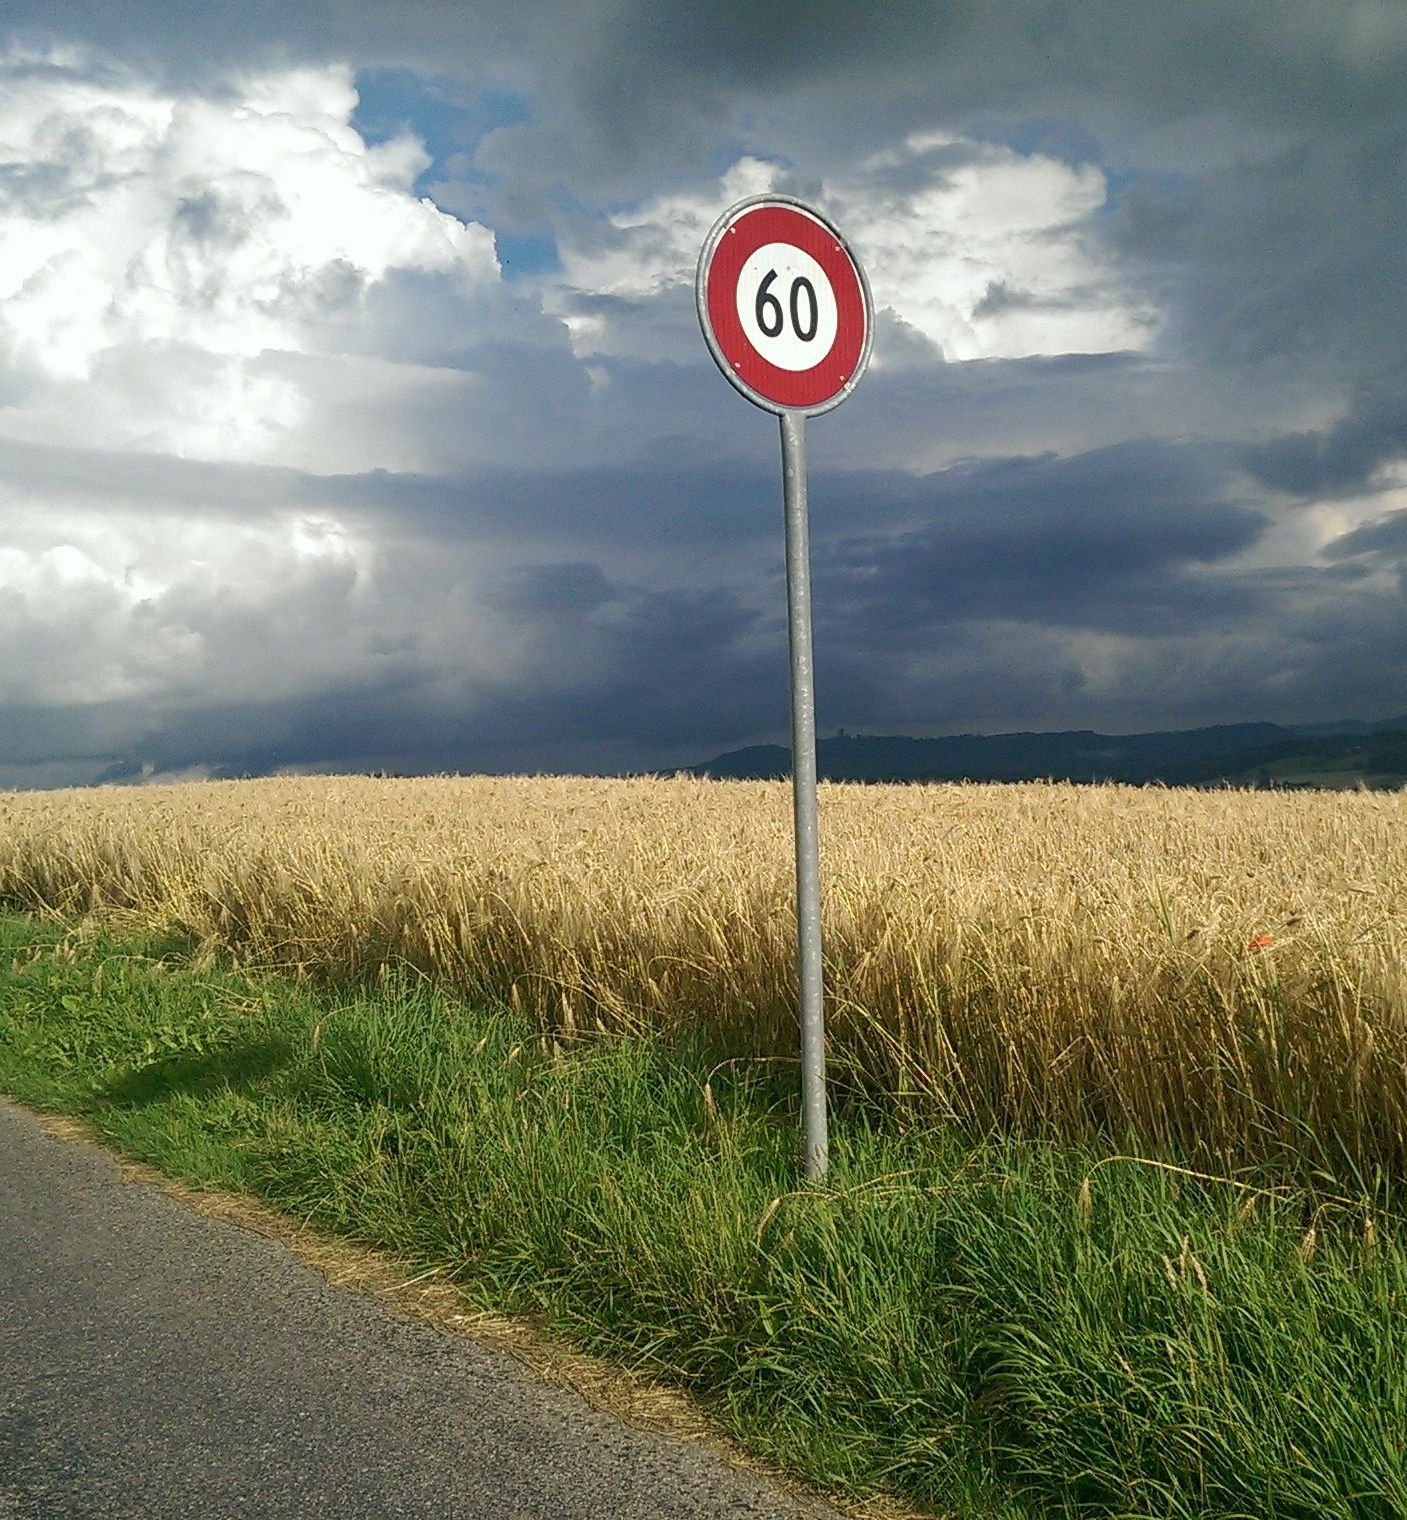
\includegraphics[width=\textwidth]{road}
		\caption*{Input image}
	\end{subfigure}
	
	\vspace{3mm}
	\begin{subfigure}[h]{0.48\textwidth}
		\centering
		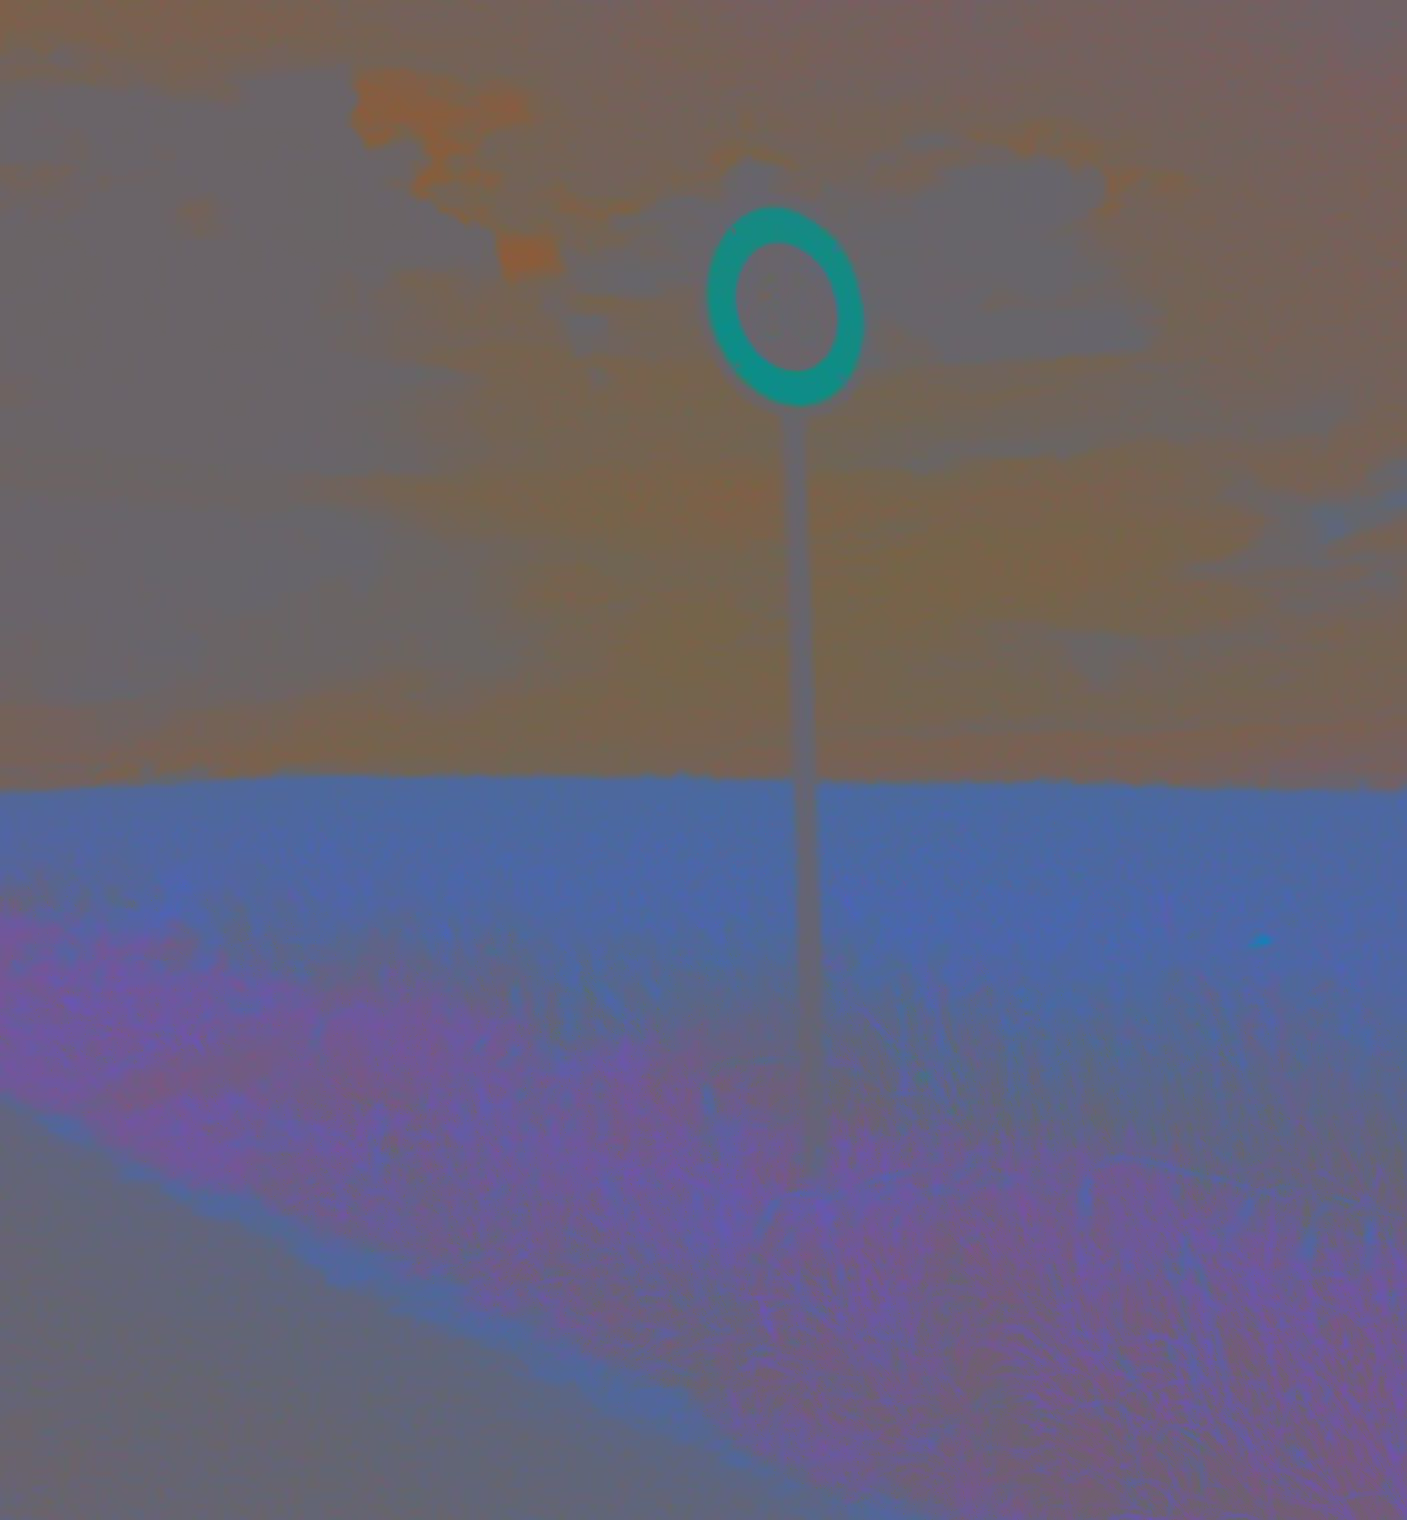
\includegraphics[width=\textwidth]{road_inv}
		\caption*{Inverted image}
	\end{subfigure}
	~
	\begin{subfigure}[h]{0.48\textwidth}
		\centering
		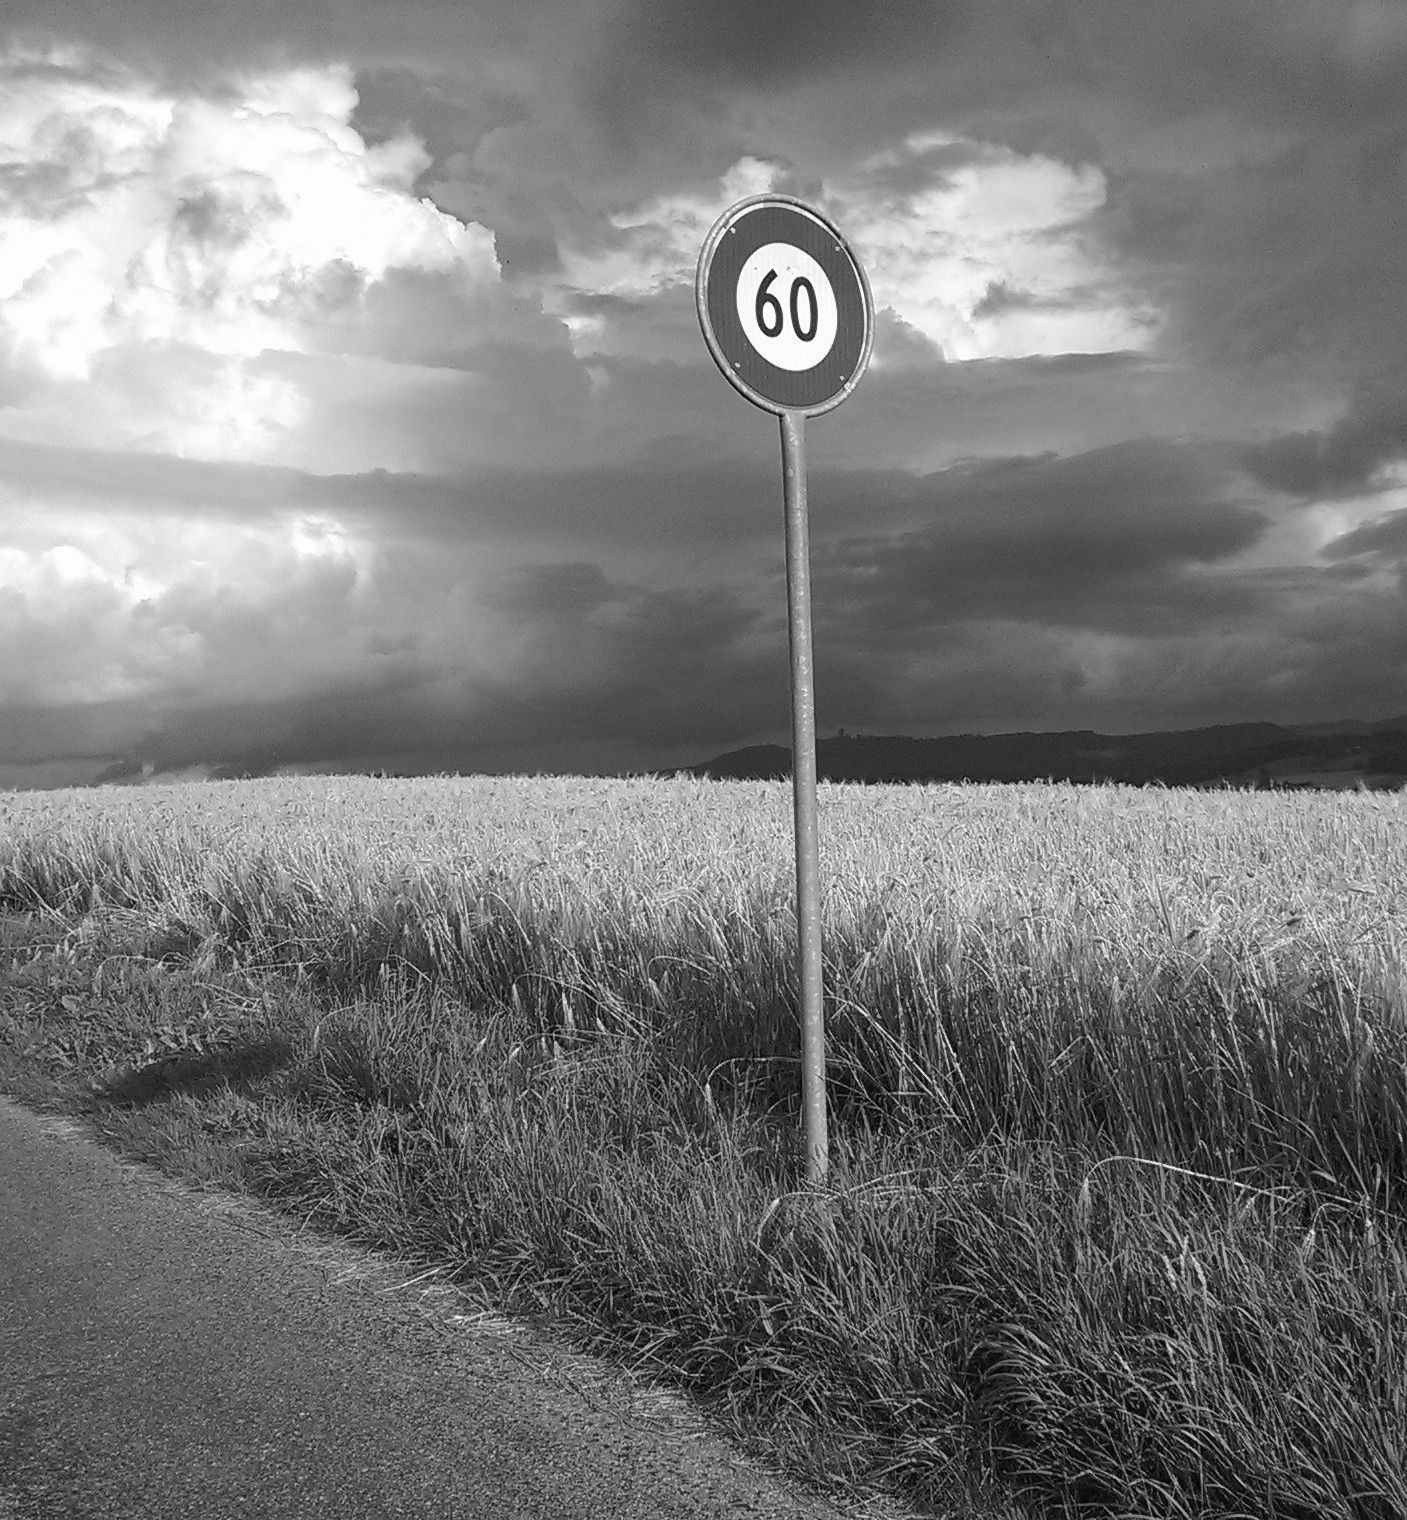
\includegraphics[width=\textwidth]{road_gray}
		\caption*{Gray-scale image}
	\end{subfigure}	
\caption{The spanish castle illusion with the example of a photograph captured near Bern in July 2014.}
\label{fig:road}
\end{figure}

\begin{figure}[H]
	%\centering
	\begin{subfigure}[h]{0.24\textwidth}
		\centering
		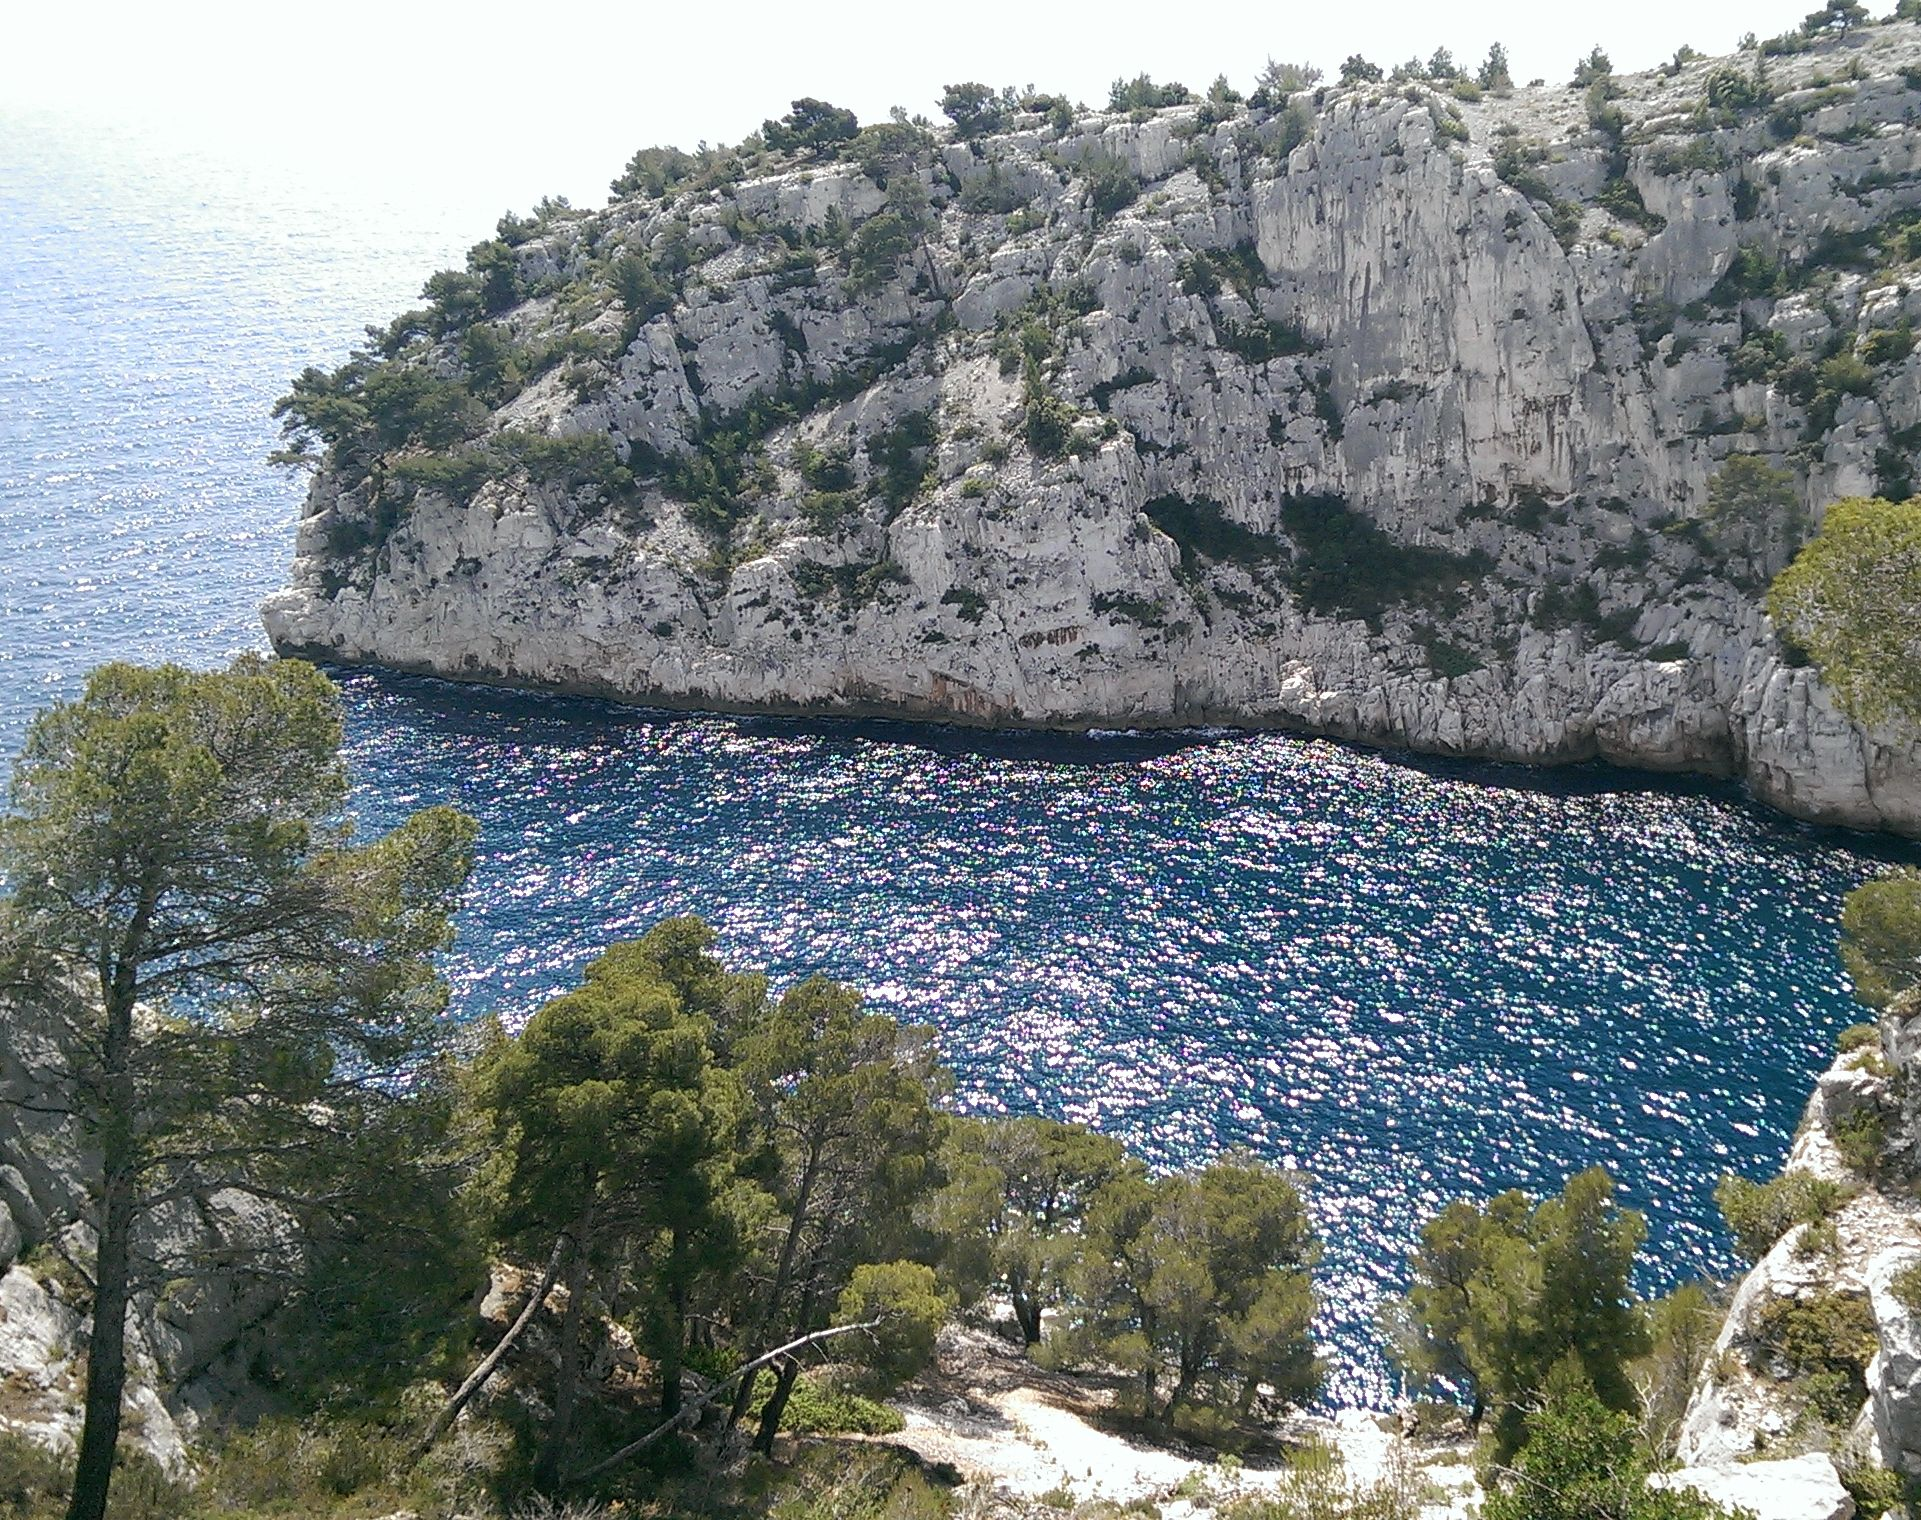
\includegraphics[width=\textwidth]{calanque}
		\caption*{Input image}
	\end{subfigure}
	
	\vspace{3mm}
	\begin{subfigure}[h]{0.48\textwidth}
		\centering
		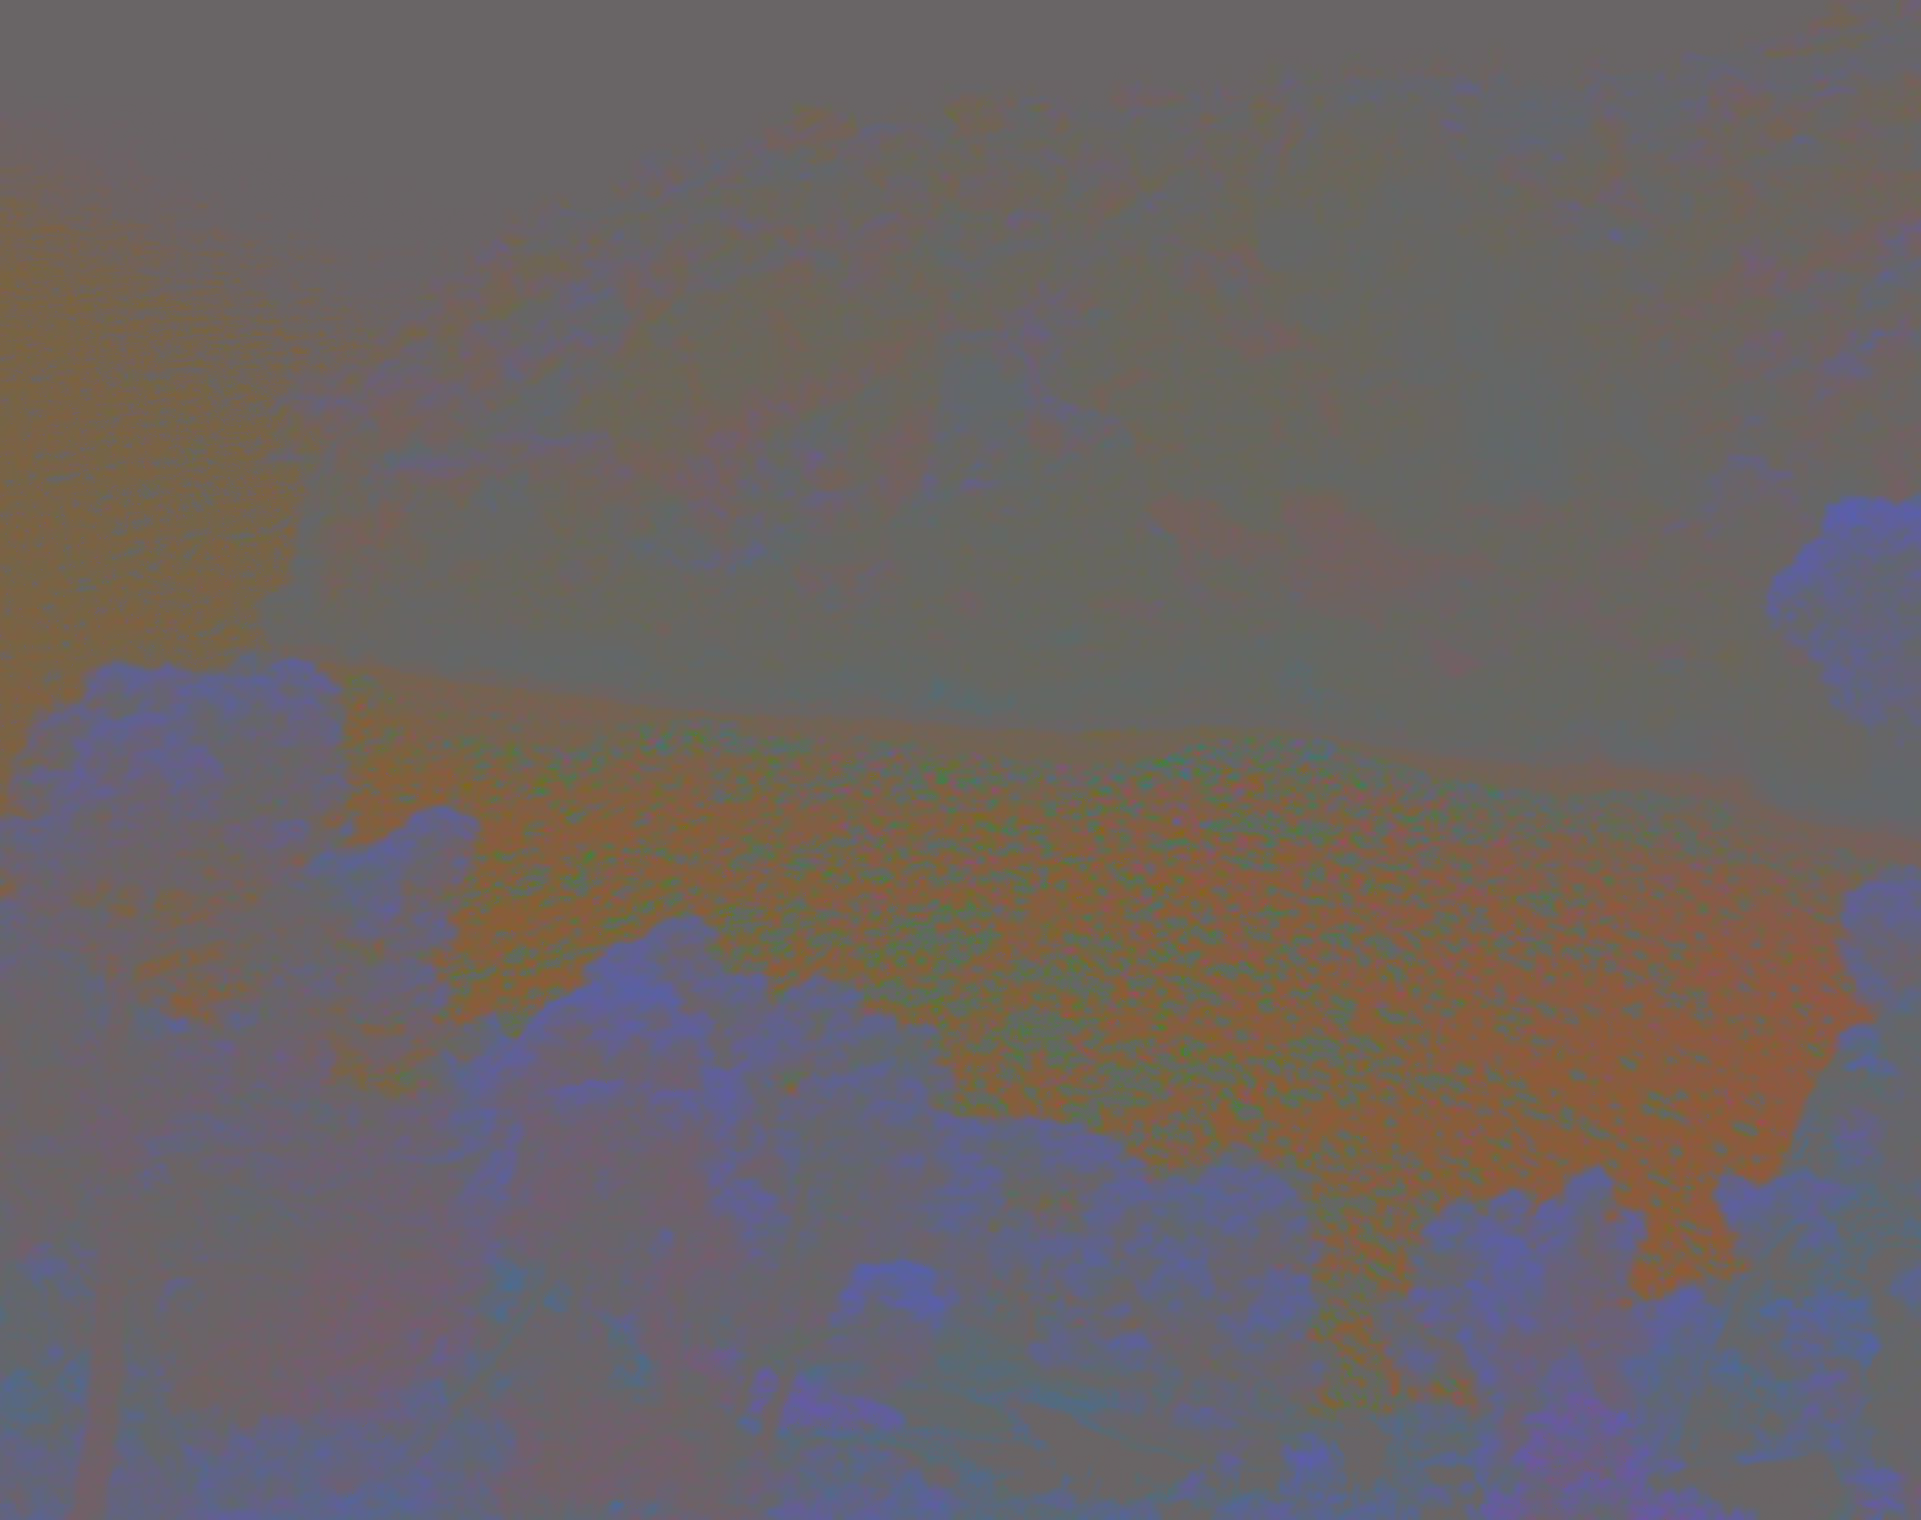
\includegraphics[width=\textwidth]{calanque_inv}
		\caption*{Inverted image}
	\end{subfigure}
	~
	\begin{subfigure}[h]{0.48\textwidth}
		\centering
		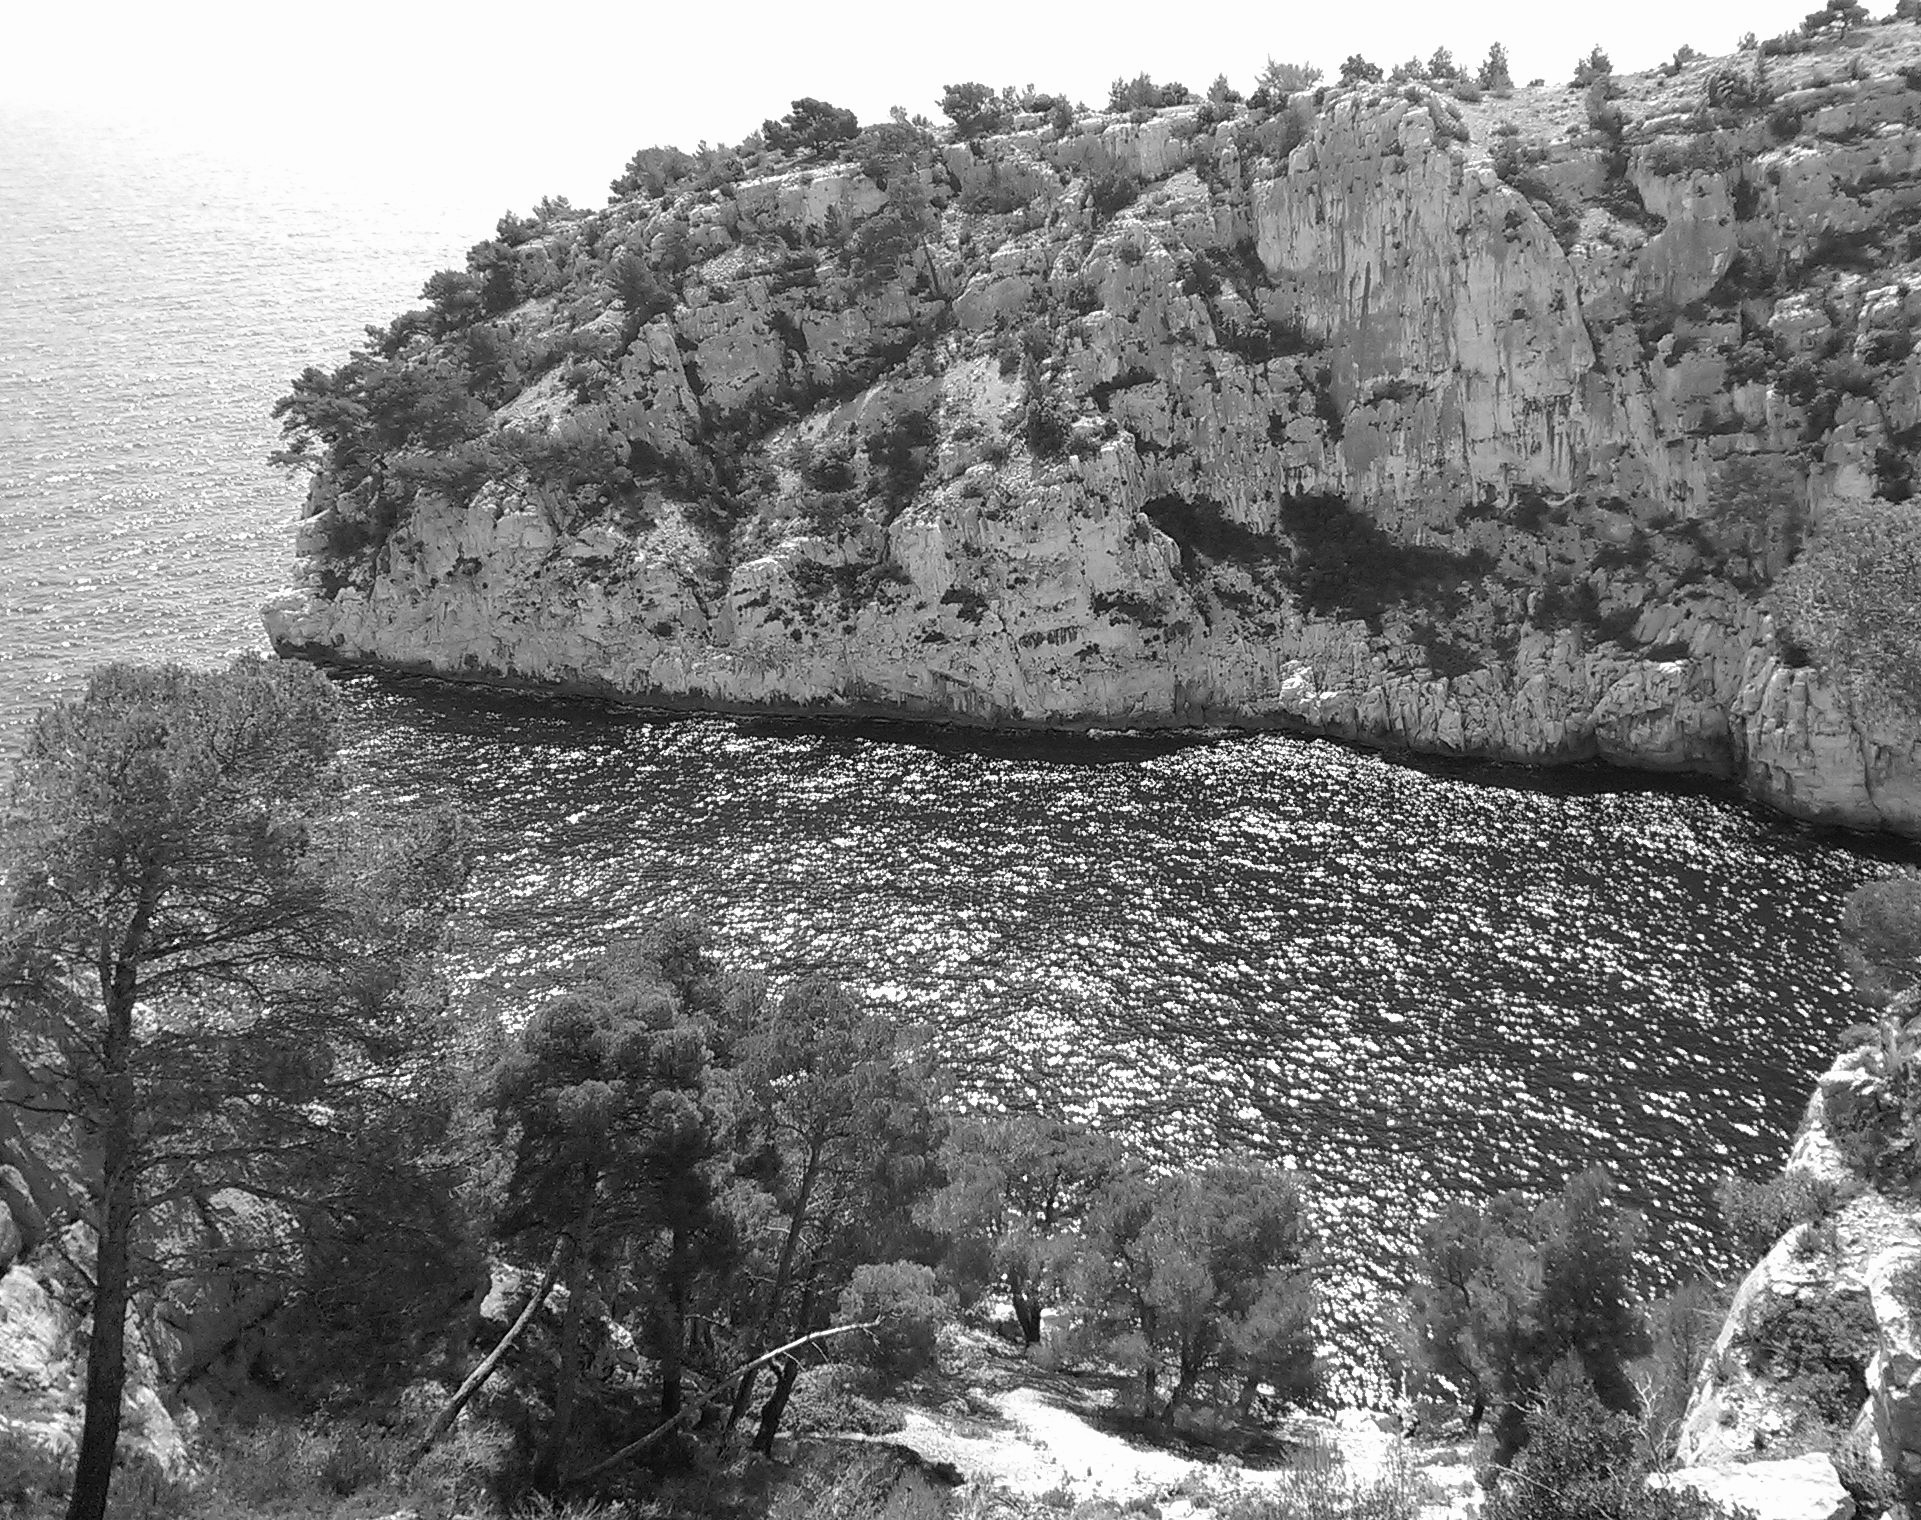
\includegraphics[width=\textwidth]{calanque_gray}
		\caption*{Gray-scale image}
	\end{subfigure}	
\caption{The spanish castle illusion with the example of a photograph captured near Cassis in May 2014.}
\label{fig:calanque}
\end{figure}

\section{Processing RAW Images}

\begin{figure}[H]
	\centering
	\vspace{3mm}
	\begin{subfigure}[h]{0.48\textwidth}
		\centering
		\includegraphics[width=\textwidth]{raw_forest_input}
		\caption*{Input}
	\end{subfigure}
	~
	\begin{subfigure}[h]{0.48\textwidth}
		\centering
		\includegraphics[width=\textwidth]{raw_forest_demosaiced_linear}
		\caption*{Demosaiced}
	\end{subfigure}	
\caption{Left: Input RAW data. Every pixel only contains the red, green or blue value, but never more than one. Therefore it can be represented by a gray-scale image. Right: Reconstructed (demosaiced) RGB image (bilinear filtering).}
\label{fig:demosaicLinForest}
\end{figure}
\subsection*{With or without filtering?}
The output image from Figure \ref{fig:demosaicLinForest} was generated using simple bilinear interpolation of the separate color channels. However, this approach may lead to artifacts called \emph{color fringing}. To address these artifacts, we filtered the interpolated image with a median filter. Some examples are visible in Figure \ref{fig:compareDemosaicing}. 
Using a large enough filter kernel of e.g.\ 5x5, we managed to get rid of a major part of the problems in our test image.
\begin{figure}[H]
	\centering
	\begin{subfigure}[h]{0.48\textwidth}
		\centering
		
\includegraphics[width=\textwidth]{black_and_white_bilinear_interpolated}
		\caption*{Bilinear interpolation}
	\end{subfigure}
	~
	\begin{subfigure}[h]{0.48\textwidth}
		\centering
		
\includegraphics[width=\textwidth]{black_and_white_median_filtered_3x3}
		\caption*{3x3 median filtered}
	\end{subfigure}	
	
	\vspace{3mm}
	\centering
	\begin{subfigure}[h]{0.32\textwidth}
		\centering
		
\includegraphics[width=\textwidth]{black_and_white_bilinear_interpolated_zoom}
		\caption*{Zoom bilinear}
	\end{subfigure}
	\begin{subfigure}[h]{0.32\textwidth}
		\centering
		
\includegraphics[width=\textwidth]{black_and_white_median_filtered_3x3_zoom}
		\caption*{Zoom 3x3 median}
	\end{subfigure}
	\begin{subfigure}[h]{0.32\textwidth}
		\centering
		
\includegraphics[width=\textwidth]{black_and_white_median_filtered_5x5_zoom}
		\caption*{Zoom 5x5median}
	\end{subfigure}
\caption{Comparison between bilinear interpolation and median filtering.}
\label{fig:compareDemosaicing}
\end{figure}
\section{Color Balancing}

\begin{figure}[H]
	%\centering
	\begin{subfigure}[h]{0.24\textwidth}
		\centering
		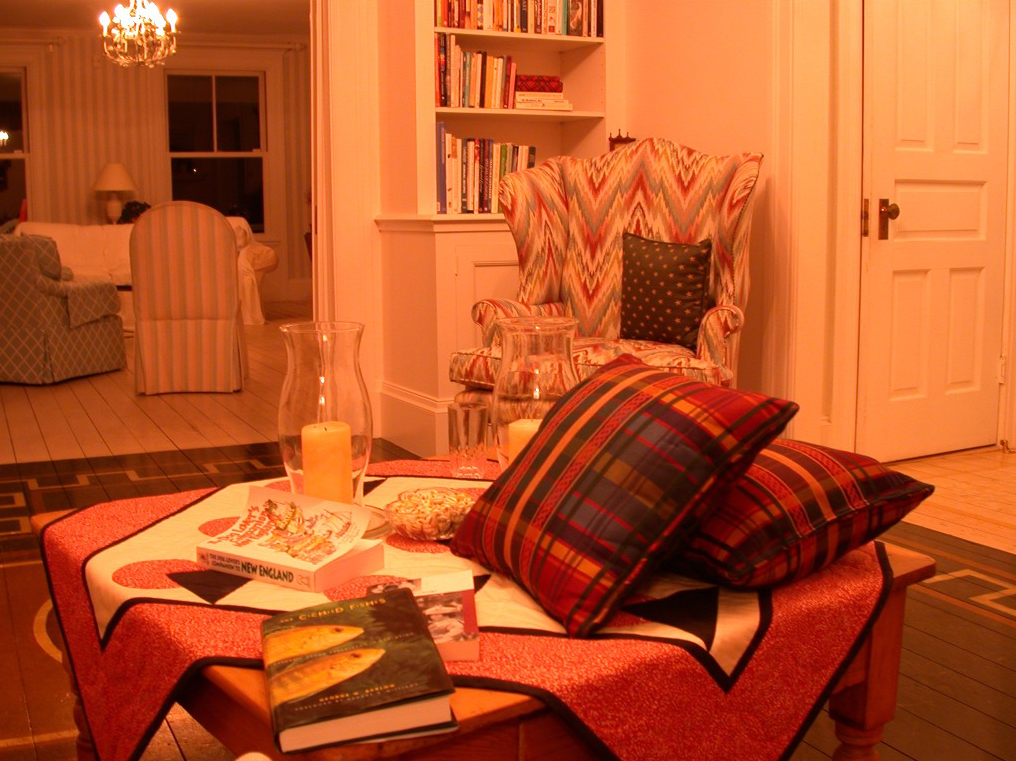
\includegraphics[width=\textwidth]{interior}
		\caption*{Input image}
	\end{subfigure}
	
	\vspace{3mm}
	\begin{subfigure}[h]{0.48\textwidth}
		\centering
		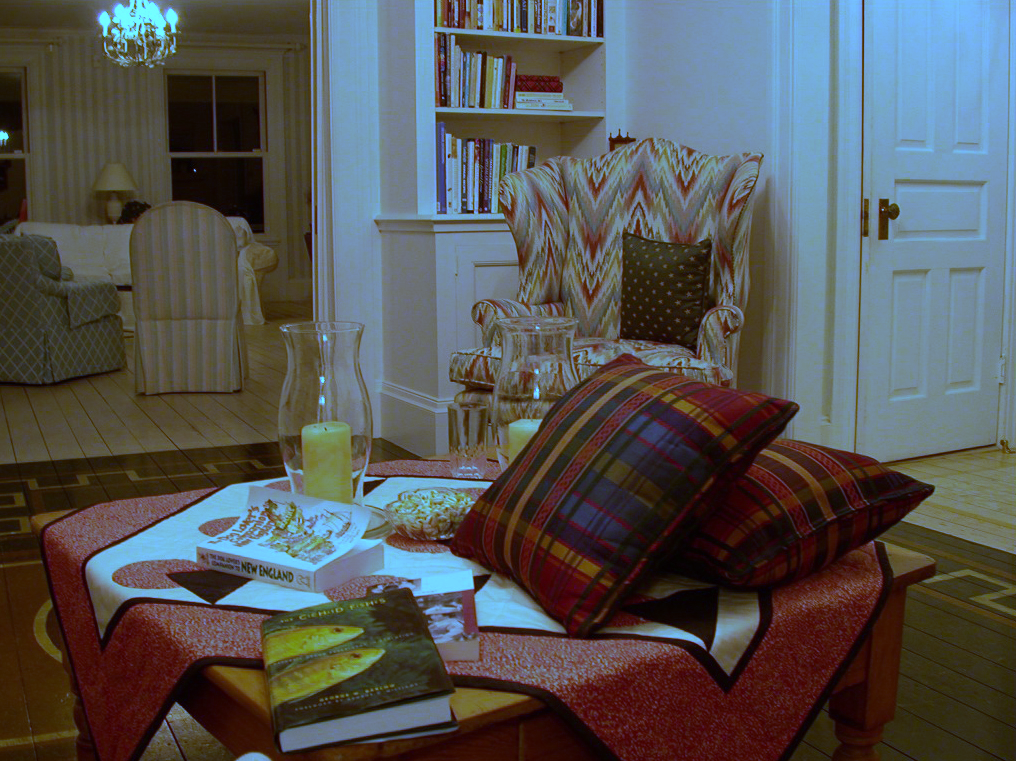
\includegraphics[width=\textwidth]{interior_gray-world1}
		\caption*{Gray world assumption}
	\end{subfigure}
	~
	\begin{subfigure}[h]{0.48\textwidth}
		\centering
		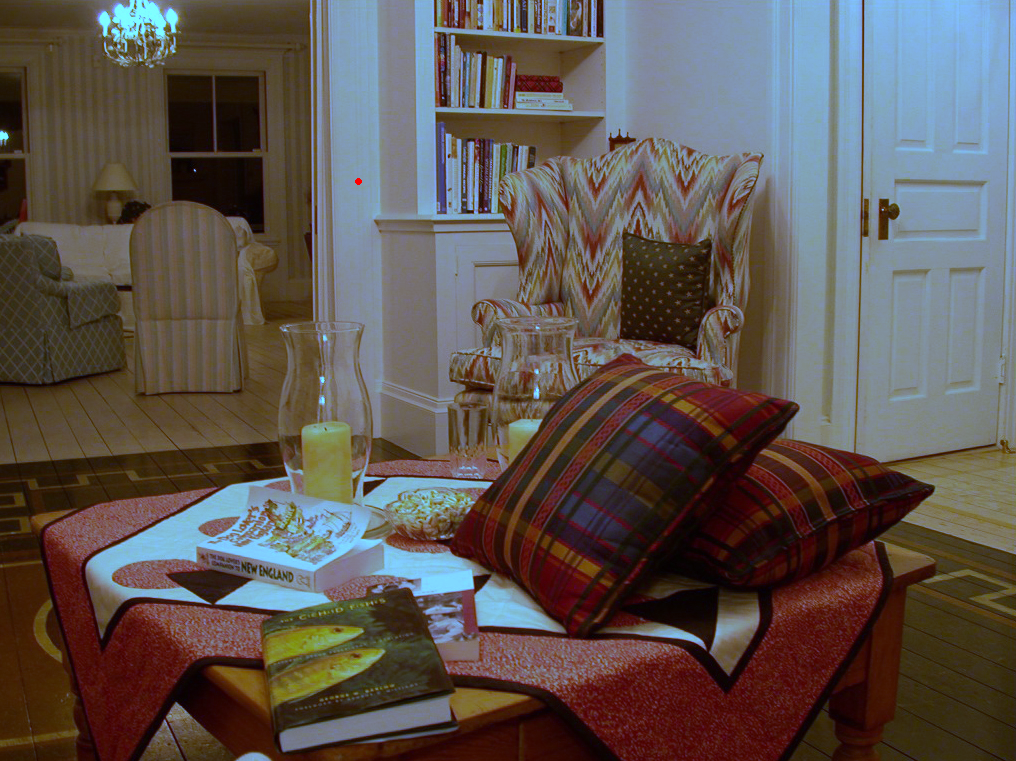
\includegraphics[width=\textwidth]{interior_manual1}
		\caption*{Manual white balancing}
	\end{subfigure}	
\caption{A reddish picture of the interior, balanced with respect to the gray world assumption (left) and a manually chosen pixel (right), marked with a red dot.}
\label{fig:interior-balance}
\end{figure}

\begin{figure}[H]
	\centering
	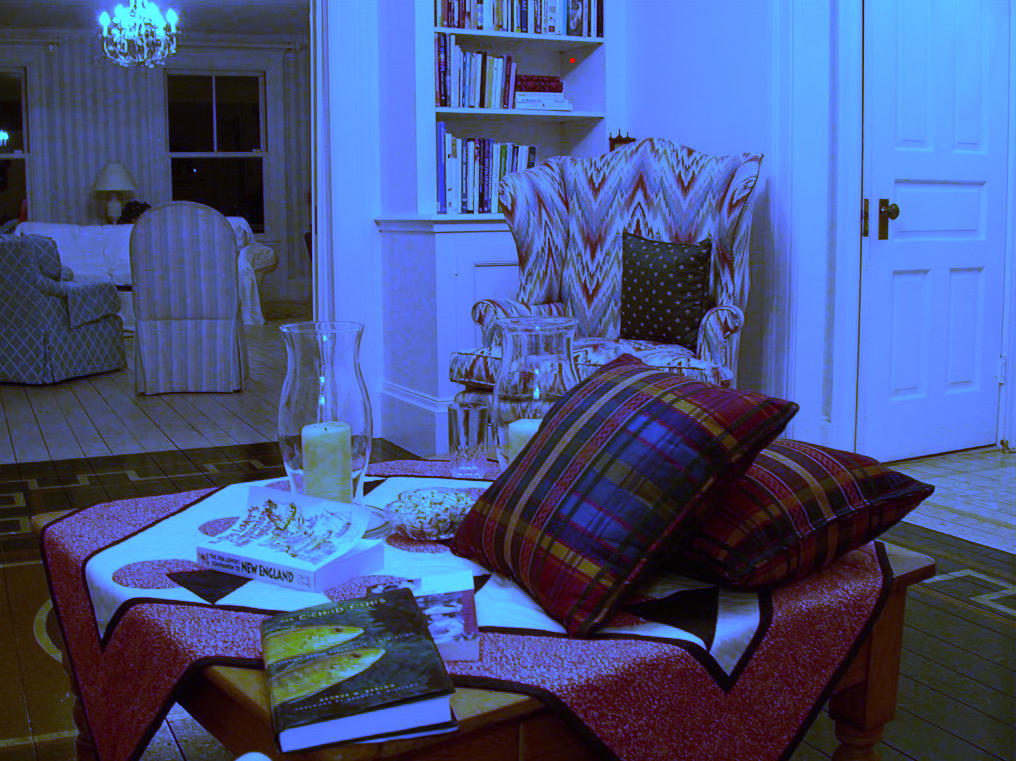
\includegraphics[width=\textwidth]{interior_manual_fail1}
\caption{A failure case of the manual white balancing: When a non-representative pixel is chosen, the color balancing does not work appropriately. In the above example, the chosen pixel is actually supposed to represent white color, but is in shadow or in more reddish regions and therefore look a bit different from the ``usual'' white pixels. The chosen pixel is indicated with a small red dot.}
\label{fig:manual-fail}
\end{figure}

\begin{figure}[H]
	%\centering
	\begin{subfigure}[h]{0.24\textwidth}
		\centering
		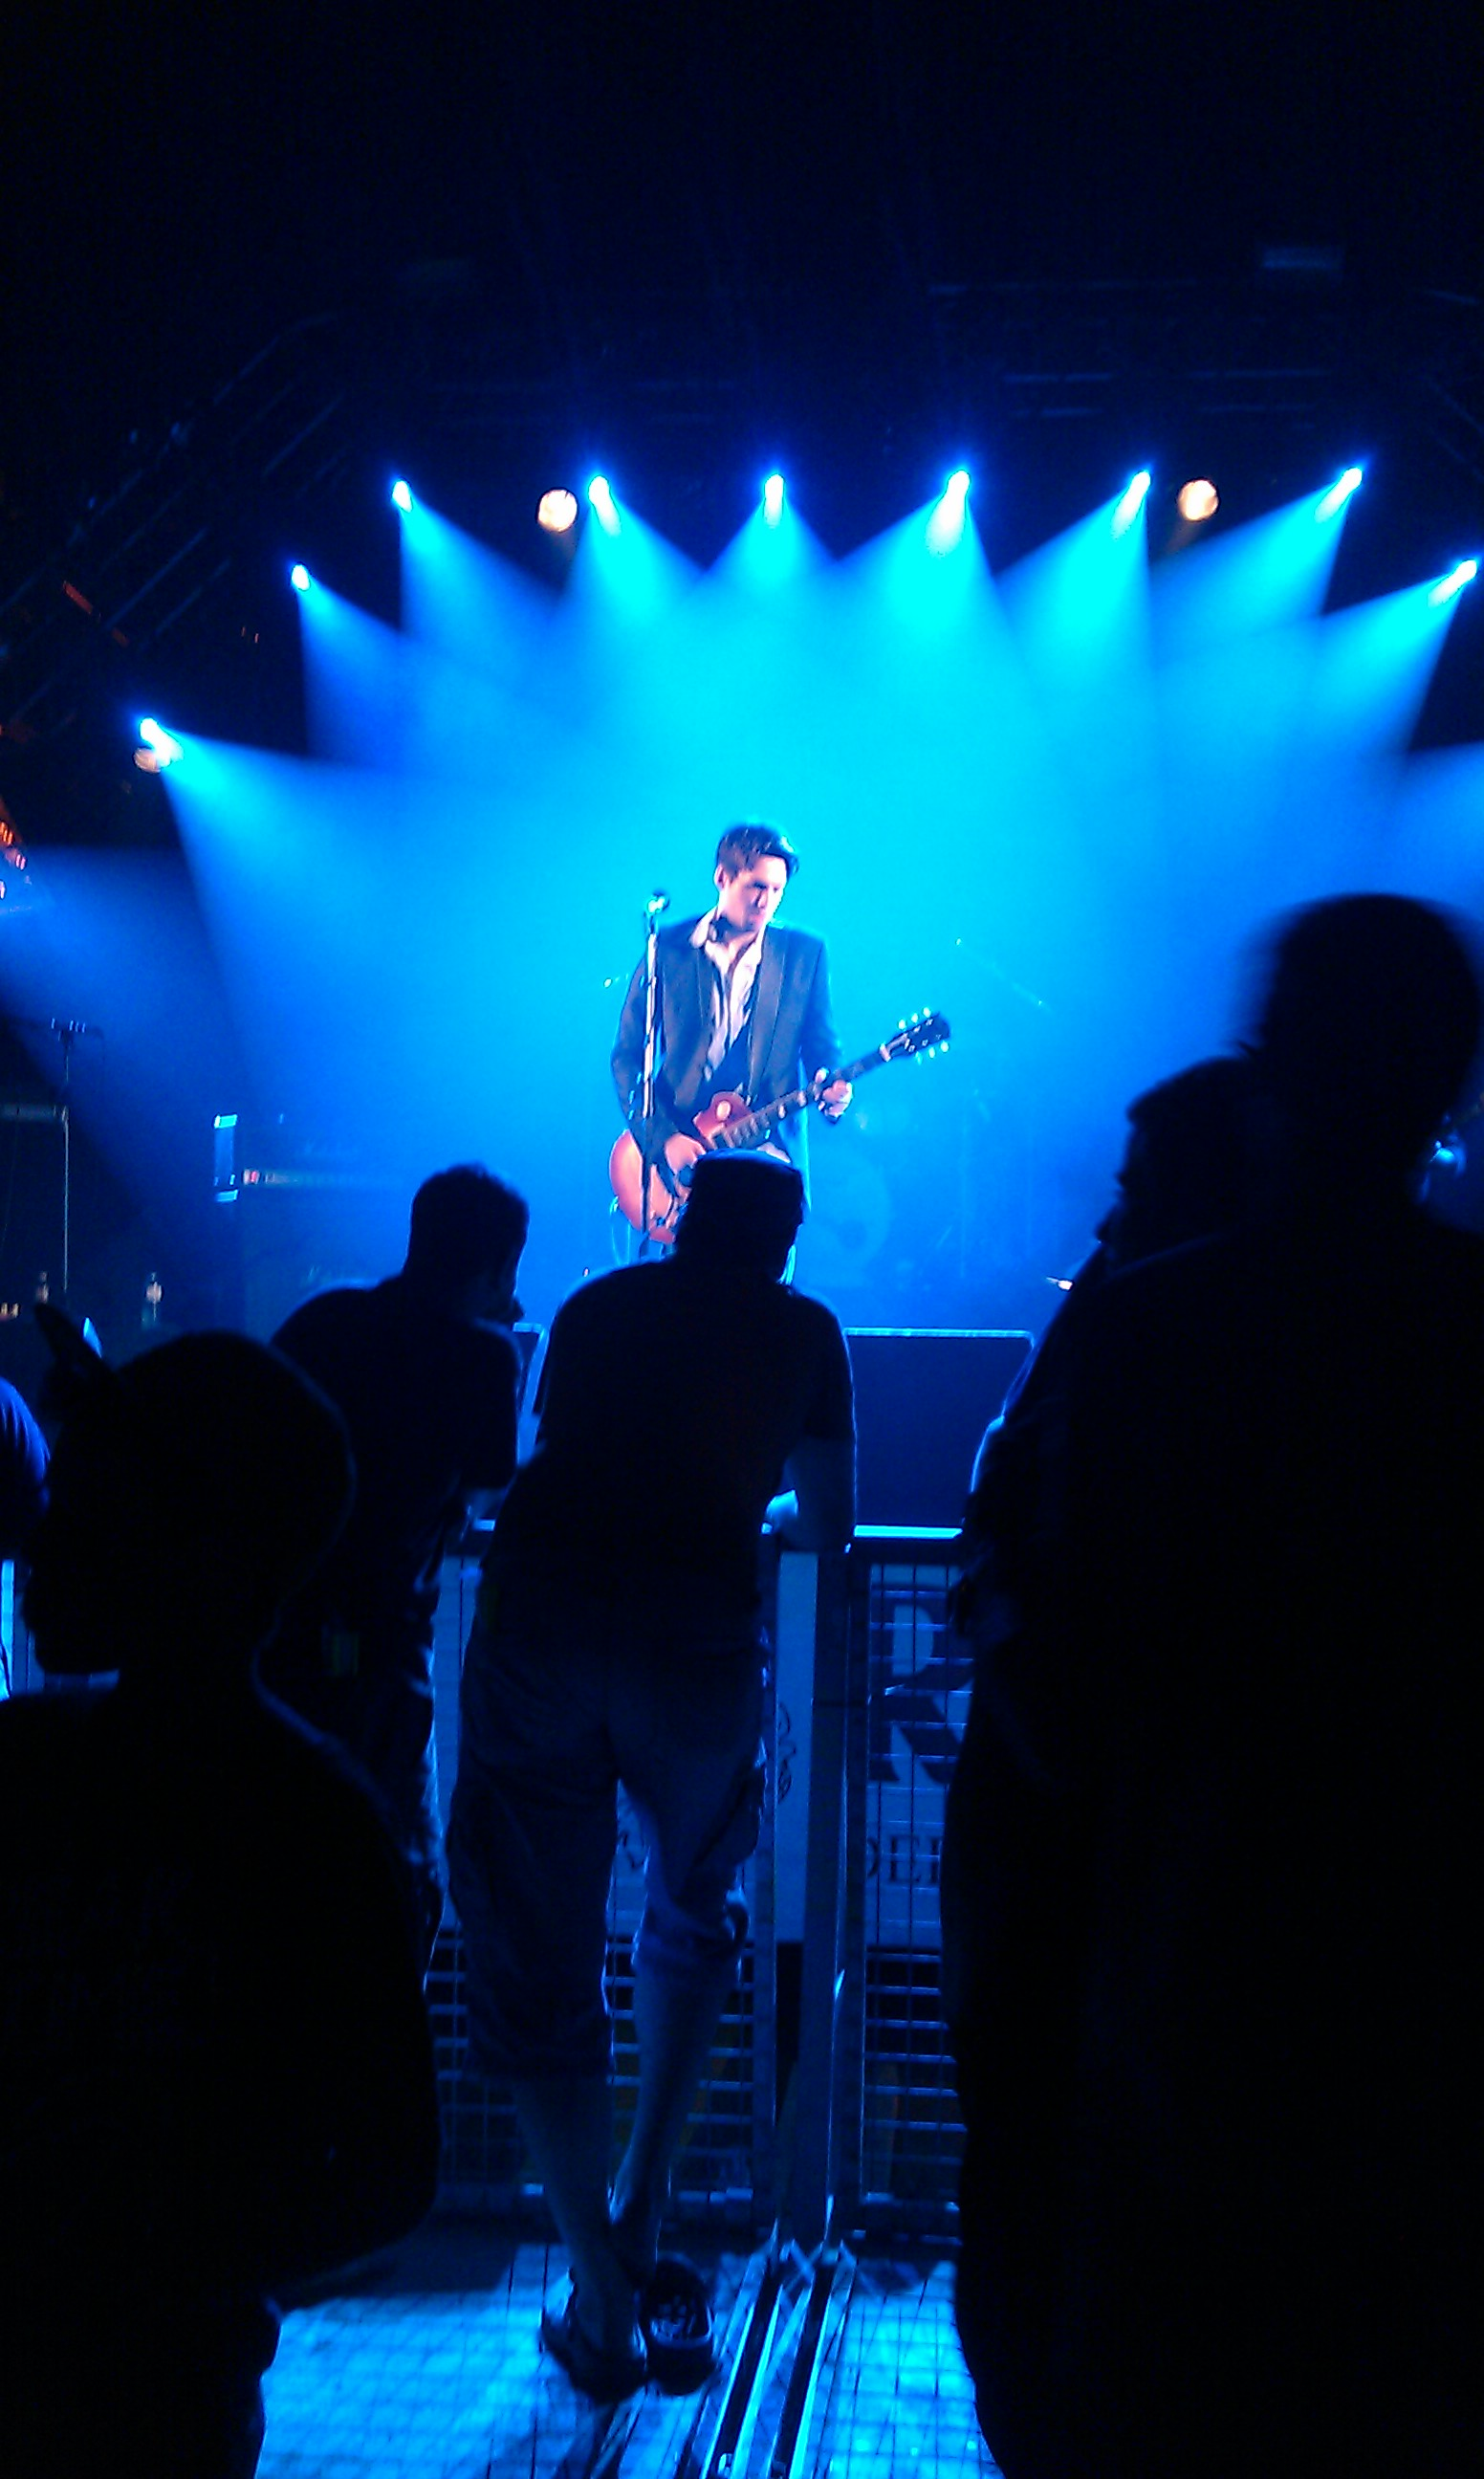
\includegraphics[width=\textwidth]{concert}
		\caption*{Input image}
	\end{subfigure}
	
	\vspace{3mm}
	\begin{subfigure}[h]{0.48\textwidth}
		\centering
		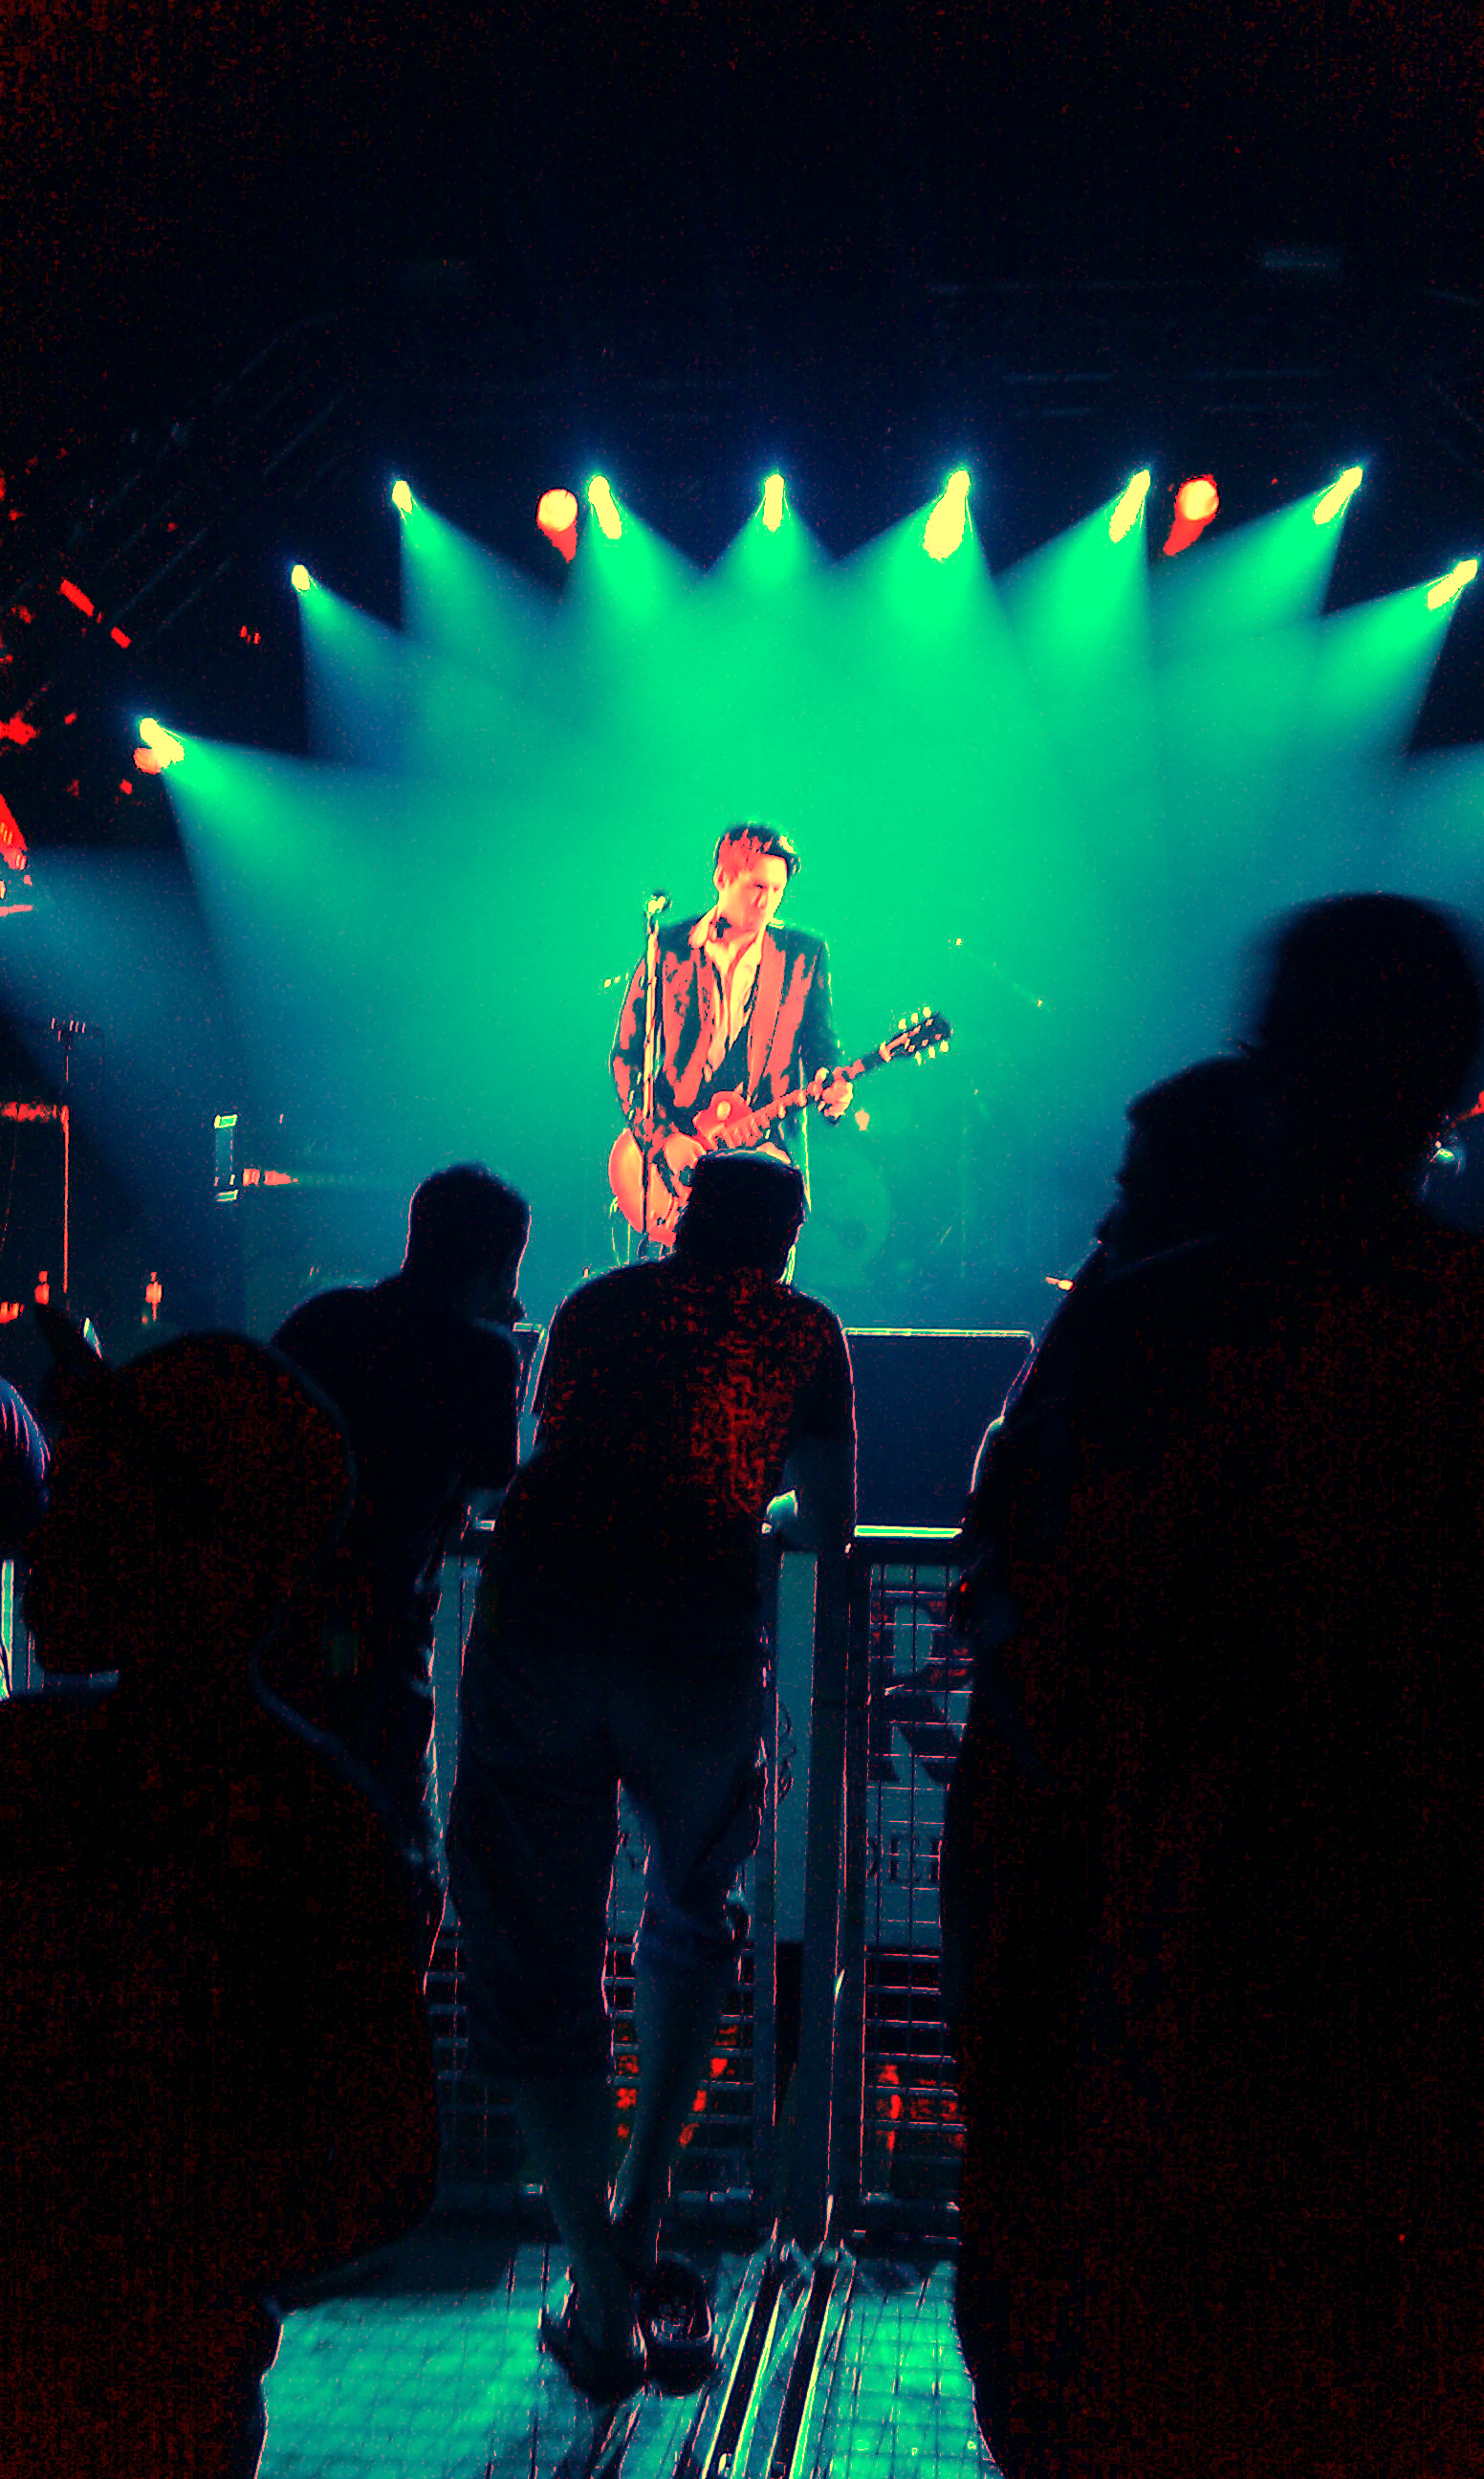
\includegraphics[width=\textwidth]{concert_gray-world}
		\caption*{Gray world assumption}
	\end{subfigure}
	~
	\begin{subfigure}[h]{0.48\textwidth}
		\centering
		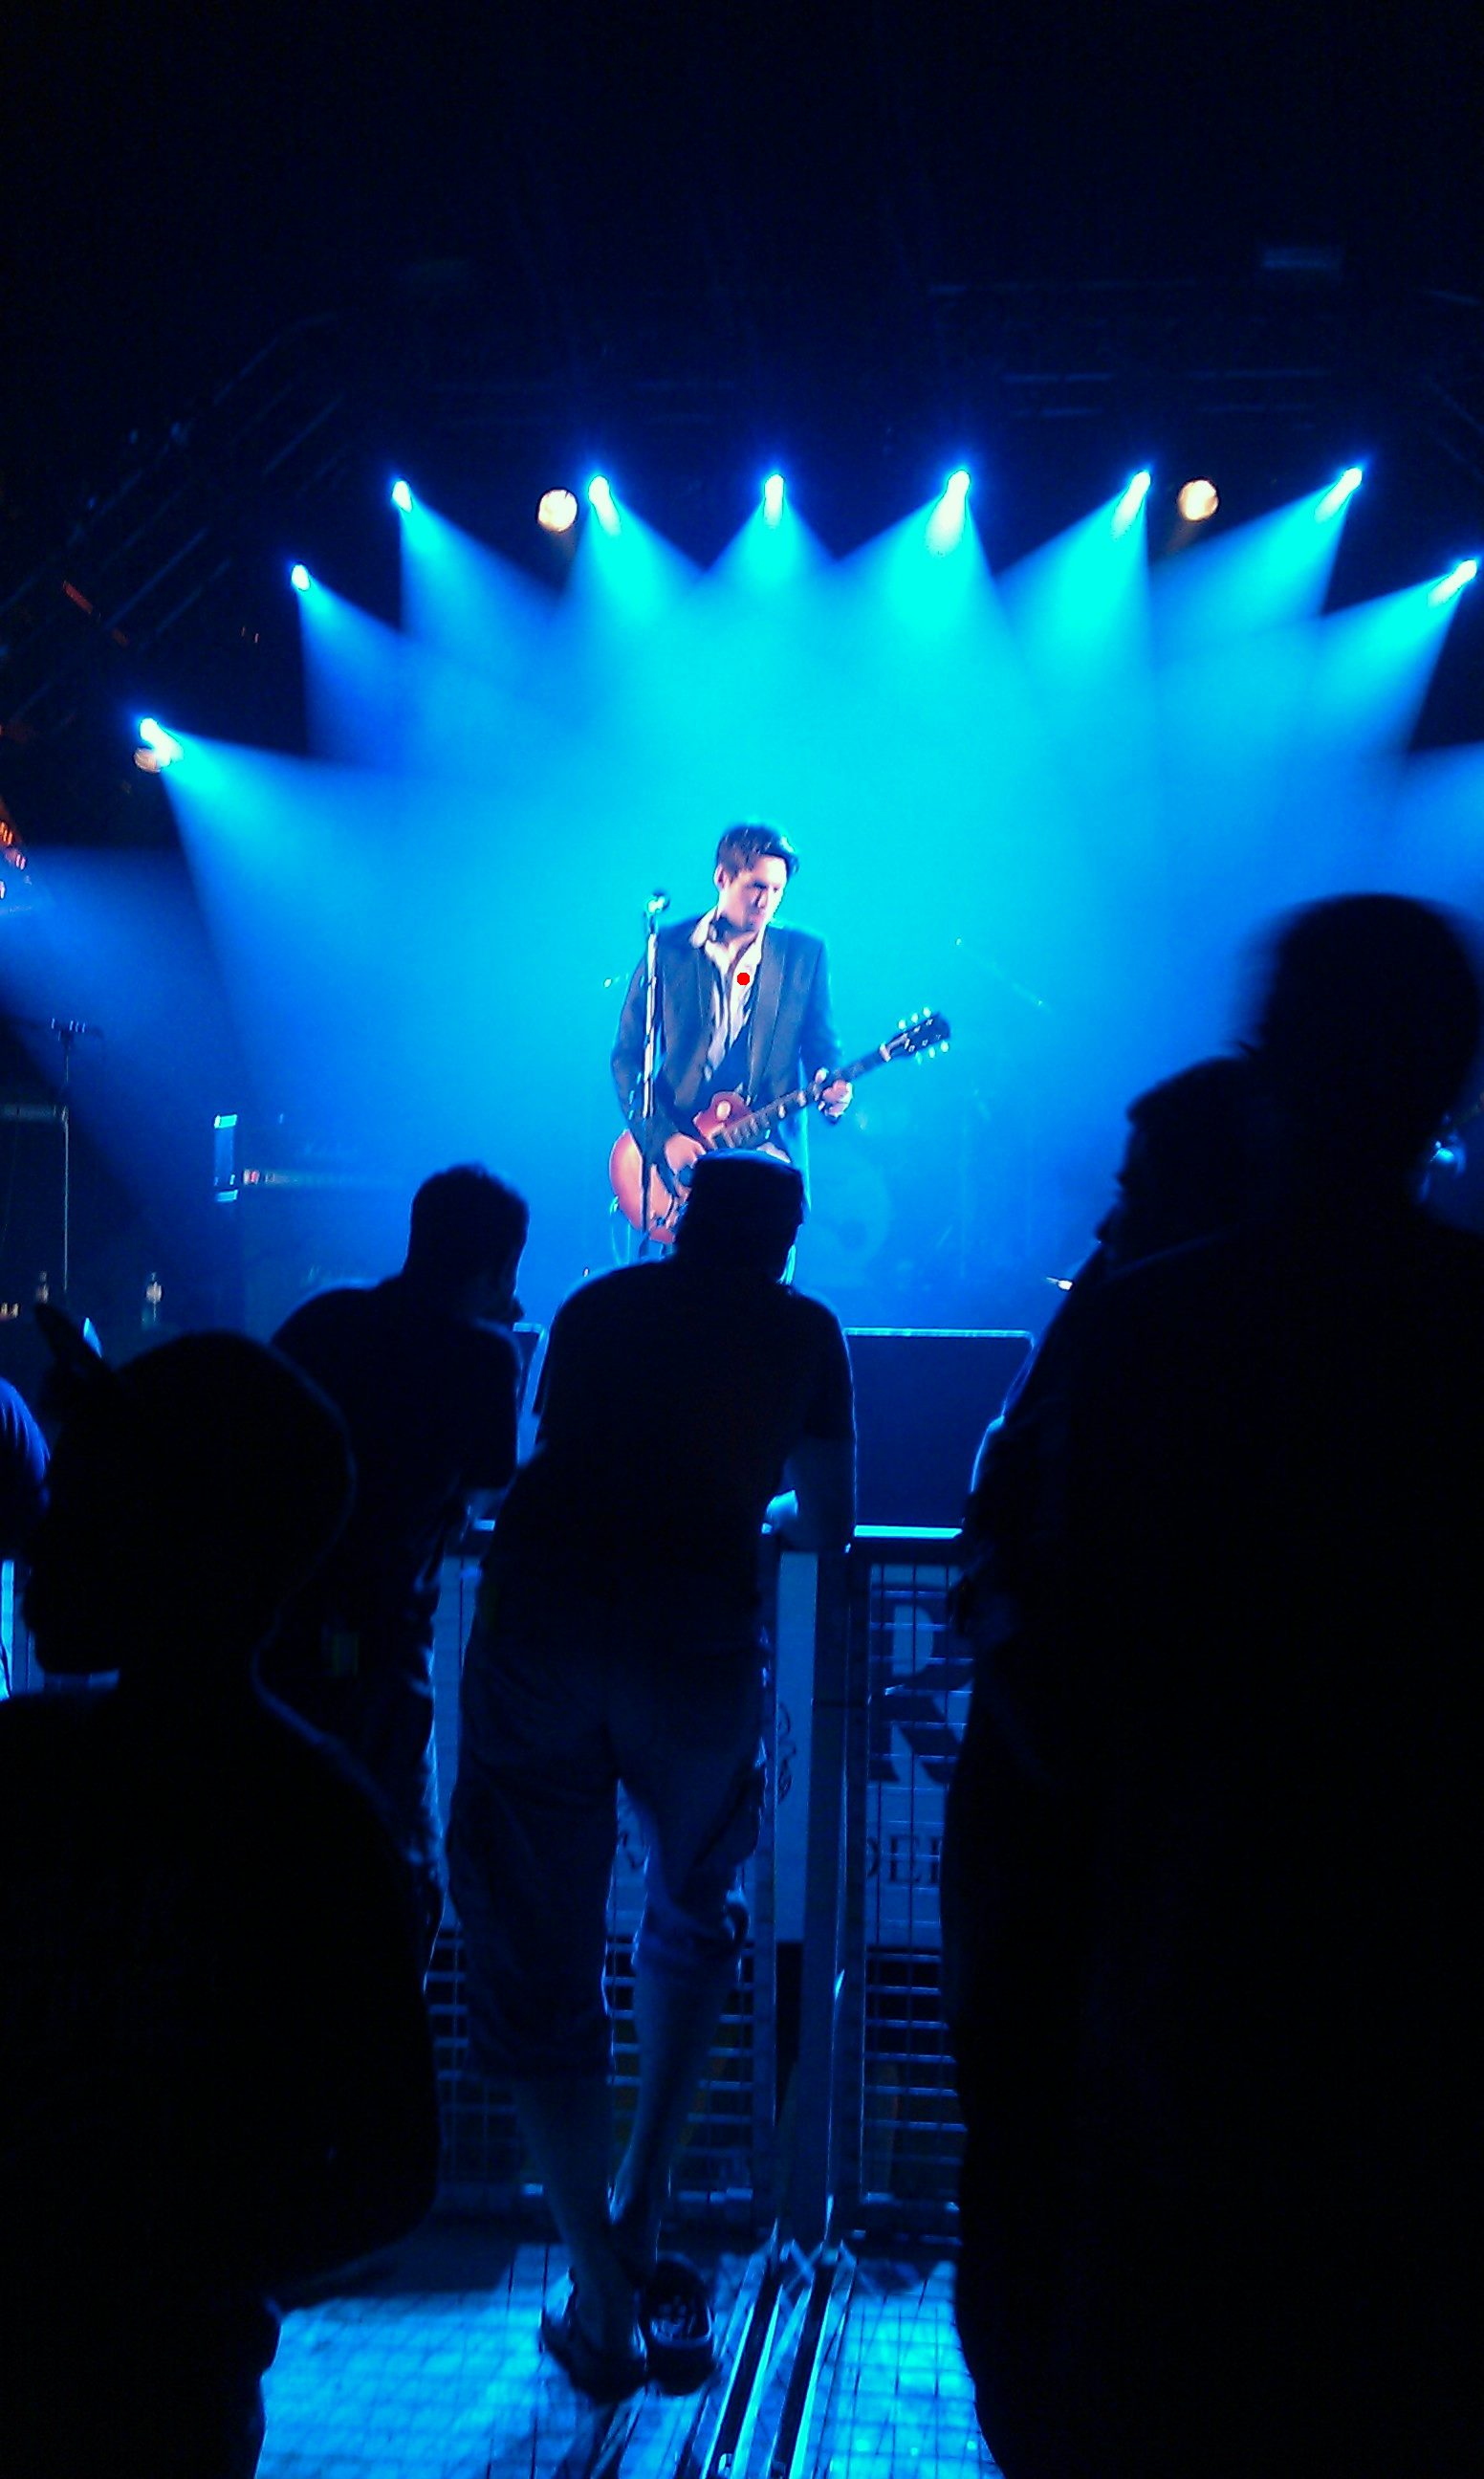
\includegraphics[width=\textwidth]{concert_manual}
		\caption*{Manual white balancing}
	\end{subfigure}	
\caption{A failure case of the gray world assumption: When one color actually \textit{is} overpresent in a scene, then the gray world assumption is obviously wrong and the corresponding balancing strategy will not preserve the desired colors. Manually choosing a pixel might in this case be better.}
\label{fig:concert-balance}
\end{figure}

\section{Global Contrast Adjustment}
\begin{figure}[H]
	%\centering
	\begin{subfigure}[h]{0.48\textwidth}
		\centering
		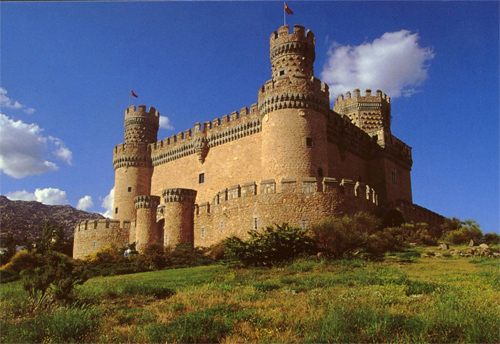
\includegraphics[width=\textwidth]{linearContrast_input1}
		\caption*{Input image}
	\end{subfigure}
	~
	\begin{subfigure}[h]{0.48\textwidth}
		\centering
		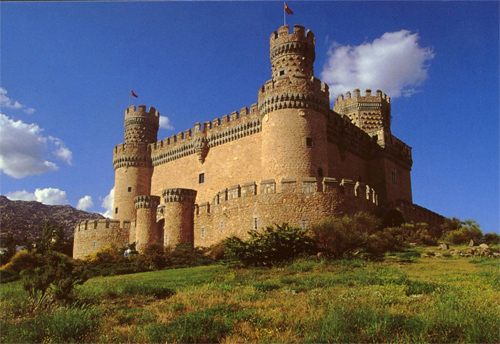
\includegraphics[width=\textwidth]{linearContrast_output1}
		\caption*{Gray world assumption}
	\end{subfigure}
	
	\vspace{3mm}
	\begin{subfigure}[h]{0.48\textwidth}
		\centering
		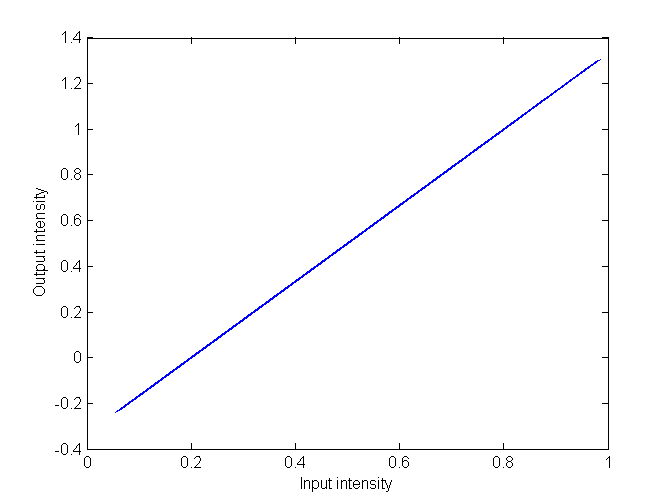
\includegraphics[width=\textwidth]{linearContrast_plot1}
		\caption*{Intensity plot}
	\end{subfigure}	
\caption{Reproduced the example image from the slides; Mapped [0.2,0.8] to [0,1] in the Spanish Castle image.}
\label{fig:contrast-1}
\end{figure}

\section{Global Contrast Adjustment}
\begin{figure}[H]
	%\centering
	\begin{subfigure}[h]{0.48\textwidth}
		\centering
		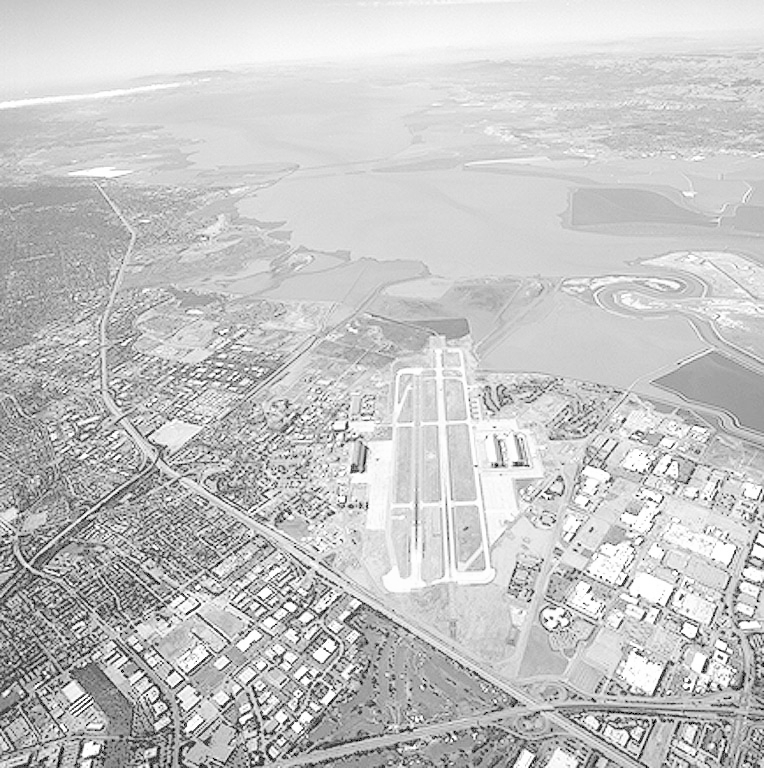
\includegraphics[width=\textwidth]{linearContrast_input2}
		\caption*{Input image}
	\end{subfigure}
	
	\vspace{3mm}
	\begin{subfigure}[h]{0.48\textwidth}
		\centering
		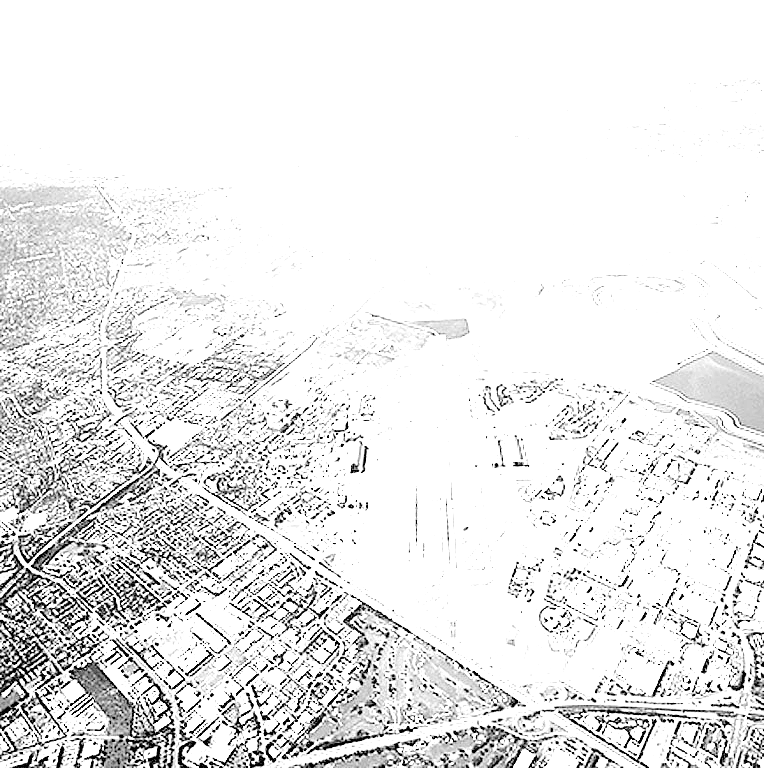
\includegraphics[width=\textwidth]{linearContrast_output2}
		\caption*{Linear scaling from [0.3,0.7] to [0,1].}
	\end{subfigure}
	~
	\begin{subfigure}[h]{0.48\textwidth}
		\centering
		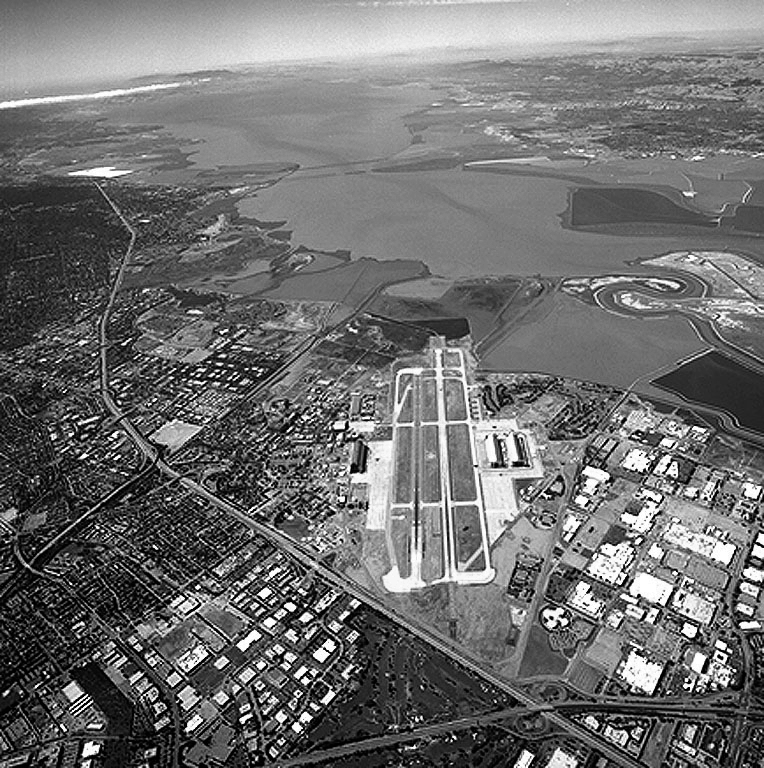
\includegraphics[width=\textwidth]{gammaContrast_output2}
		\caption*{Gamma transformation with $\gamma = 4$}
	\end{subfigure}
	
	\vspace{3mm}
	\begin{subfigure}[h]{0.48\textwidth}
		\centering
		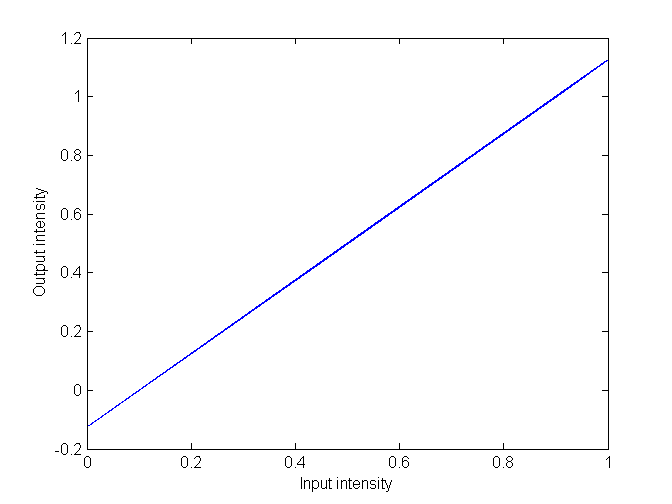
\includegraphics[width=\textwidth]{linearContrast_plot2}
		\caption*{Intensity plot}
	\end{subfigure}	
	~
	\begin{subfigure}[h]{0.48\textwidth}
		\centering
		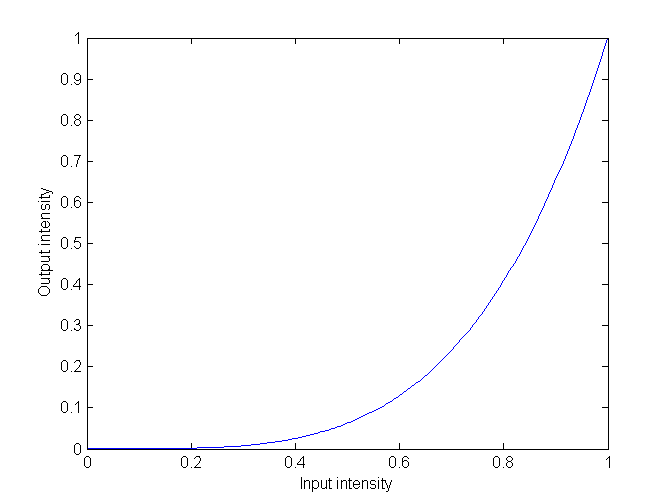
\includegraphics[width=\textwidth]{gammaContrast_plot2}
		\caption*{Intensity plot}
	\end{subfigure}	
\caption{Comparison of Contrast adjustment using linear scaling and the gamma transformation, respectively.}
\label{fig:contrast-2}
\end{figure}

\section{Bonus}
\begin{figure}[H]
	%\centering
	\begin{subfigure}[h]{0.3\textwidth}
		\centering
		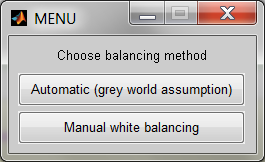
\includegraphics[width=\textwidth]{gui1}
		\caption*{Choose balancing mode}
	\end{subfigure}
	
	\vspace{3mm}
	\begin{subfigure}[h]{0.8\textwidth}
		\centering
		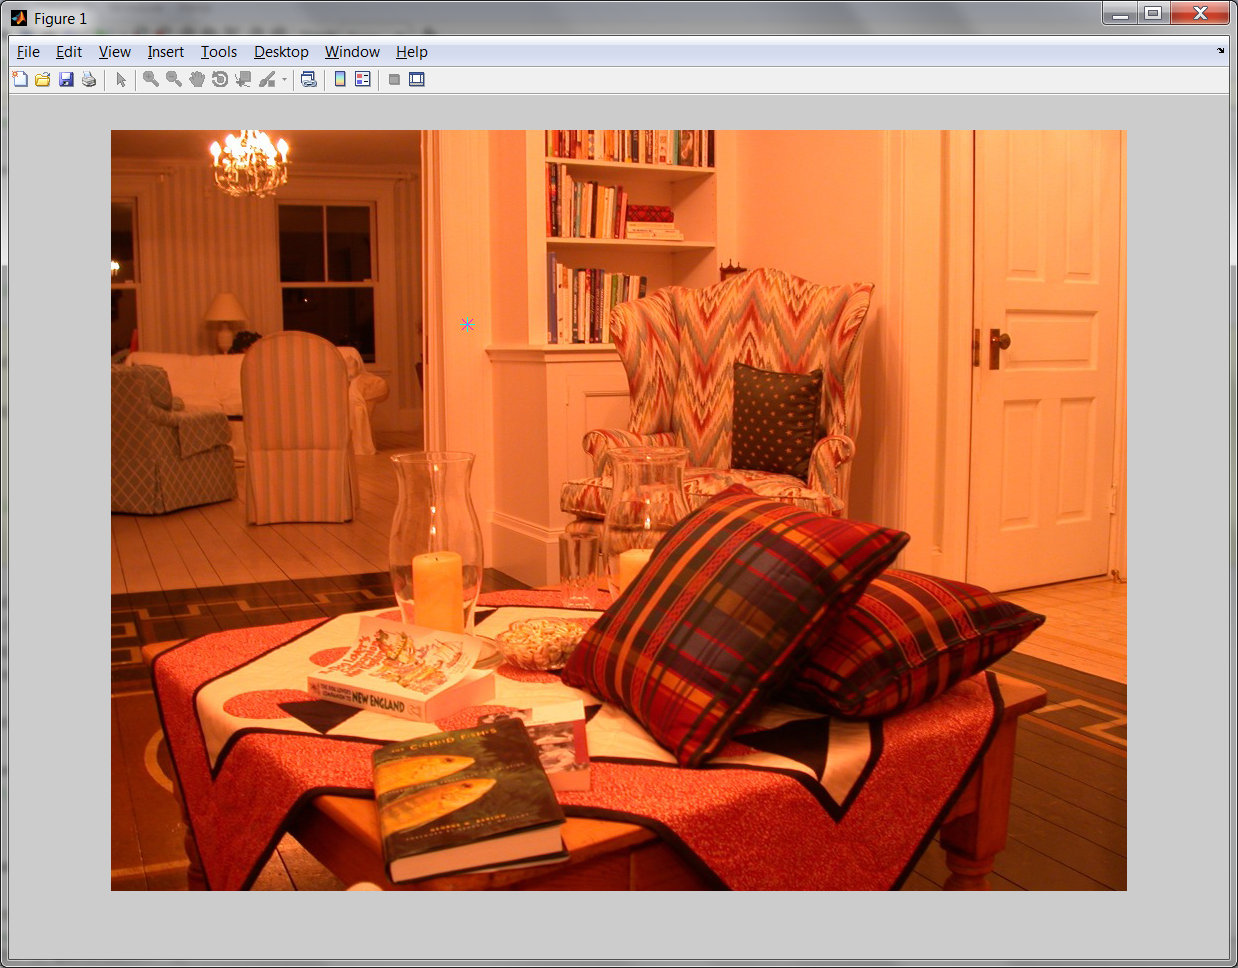
\includegraphics[width=\textwidth]{gui2}
		\caption*{Manual White balancing: Chose a pixel}
	\end{subfigure}
\caption{The small gui for the Color balancing.}
\label{fig:concert-balance}
\end{figure}
\end{document}